% Options for packages loaded elsewhere
\PassOptionsToPackage{unicode}{hyperref}
\PassOptionsToPackage{hyphens}{url}
\PassOptionsToPackage{dvipsnames,svgnames,x11names}{xcolor}
%
\documentclass[
  12pt,
  a4paper,
  DIV=11,
  numbers=noendperiod]{scrartcl}

\usepackage{amsmath,amssymb}
\usepackage{iftex}
\ifPDFTeX
  \usepackage[T1]{fontenc}
  \usepackage[utf8]{inputenc}
  \usepackage{textcomp} % provide euro and other symbols
\else % if luatex or xetex
  \usepackage{unicode-math}
  \defaultfontfeatures{Scale=MatchLowercase}
  \defaultfontfeatures[\rmfamily]{Ligatures=TeX,Scale=1}
\fi
\usepackage{lmodern}
\ifPDFTeX\else  
    % xetex/luatex font selection
\fi
% Use upquote if available, for straight quotes in verbatim environments
\IfFileExists{upquote.sty}{\usepackage{upquote}}{}
\IfFileExists{microtype.sty}{% use microtype if available
  \usepackage[]{microtype}
  \UseMicrotypeSet[protrusion]{basicmath} % disable protrusion for tt fonts
}{}
\makeatletter
\@ifundefined{KOMAClassName}{% if non-KOMA class
  \IfFileExists{parskip.sty}{%
    \usepackage{parskip}
  }{% else
    \setlength{\parindent}{0pt}
    \setlength{\parskip}{6pt plus 2pt minus 1pt}}
}{% if KOMA class
  \KOMAoptions{parskip=half}}
\makeatother
\usepackage{xcolor}
\usepackage[top=20mm,left=20mm,heightrounded]{geometry}
\setlength{\emergencystretch}{3em} % prevent overfull lines
\setcounter{secnumdepth}{-\maxdimen} % remove section numbering
% Make \paragraph and \subparagraph free-standing
\ifx\paragraph\undefined\else
  \let\oldparagraph\paragraph
  \renewcommand{\paragraph}[1]{\oldparagraph{#1}\mbox{}}
\fi
\ifx\subparagraph\undefined\else
  \let\oldsubparagraph\subparagraph
  \renewcommand{\subparagraph}[1]{\oldsubparagraph{#1}\mbox{}}
\fi

\usepackage{color}
\usepackage{fancyvrb}
\newcommand{\VerbBar}{|}
\newcommand{\VERB}{\Verb[commandchars=\\\{\}]}
\DefineVerbatimEnvironment{Highlighting}{Verbatim}{commandchars=\\\{\}}
% Add ',fontsize=\small' for more characters per line
\usepackage{framed}
\definecolor{shadecolor}{RGB}{241,243,245}
\newenvironment{Shaded}{\begin{snugshade}}{\end{snugshade}}
\newcommand{\AlertTok}[1]{\textcolor[rgb]{0.68,0.00,0.00}{#1}}
\newcommand{\AnnotationTok}[1]{\textcolor[rgb]{0.37,0.37,0.37}{#1}}
\newcommand{\AttributeTok}[1]{\textcolor[rgb]{0.40,0.45,0.13}{#1}}
\newcommand{\BaseNTok}[1]{\textcolor[rgb]{0.68,0.00,0.00}{#1}}
\newcommand{\BuiltInTok}[1]{\textcolor[rgb]{0.00,0.23,0.31}{#1}}
\newcommand{\CharTok}[1]{\textcolor[rgb]{0.13,0.47,0.30}{#1}}
\newcommand{\CommentTok}[1]{\textcolor[rgb]{0.37,0.37,0.37}{#1}}
\newcommand{\CommentVarTok}[1]{\textcolor[rgb]{0.37,0.37,0.37}{\textit{#1}}}
\newcommand{\ConstantTok}[1]{\textcolor[rgb]{0.56,0.35,0.01}{#1}}
\newcommand{\ControlFlowTok}[1]{\textcolor[rgb]{0.00,0.23,0.31}{#1}}
\newcommand{\DataTypeTok}[1]{\textcolor[rgb]{0.68,0.00,0.00}{#1}}
\newcommand{\DecValTok}[1]{\textcolor[rgb]{0.68,0.00,0.00}{#1}}
\newcommand{\DocumentationTok}[1]{\textcolor[rgb]{0.37,0.37,0.37}{\textit{#1}}}
\newcommand{\ErrorTok}[1]{\textcolor[rgb]{0.68,0.00,0.00}{#1}}
\newcommand{\ExtensionTok}[1]{\textcolor[rgb]{0.00,0.23,0.31}{#1}}
\newcommand{\FloatTok}[1]{\textcolor[rgb]{0.68,0.00,0.00}{#1}}
\newcommand{\FunctionTok}[1]{\textcolor[rgb]{0.28,0.35,0.67}{#1}}
\newcommand{\ImportTok}[1]{\textcolor[rgb]{0.00,0.46,0.62}{#1}}
\newcommand{\InformationTok}[1]{\textcolor[rgb]{0.37,0.37,0.37}{#1}}
\newcommand{\KeywordTok}[1]{\textcolor[rgb]{0.00,0.23,0.31}{#1}}
\newcommand{\NormalTok}[1]{\textcolor[rgb]{0.00,0.23,0.31}{#1}}
\newcommand{\OperatorTok}[1]{\textcolor[rgb]{0.37,0.37,0.37}{#1}}
\newcommand{\OtherTok}[1]{\textcolor[rgb]{0.00,0.23,0.31}{#1}}
\newcommand{\PreprocessorTok}[1]{\textcolor[rgb]{0.68,0.00,0.00}{#1}}
\newcommand{\RegionMarkerTok}[1]{\textcolor[rgb]{0.00,0.23,0.31}{#1}}
\newcommand{\SpecialCharTok}[1]{\textcolor[rgb]{0.37,0.37,0.37}{#1}}
\newcommand{\SpecialStringTok}[1]{\textcolor[rgb]{0.13,0.47,0.30}{#1}}
\newcommand{\StringTok}[1]{\textcolor[rgb]{0.13,0.47,0.30}{#1}}
\newcommand{\VariableTok}[1]{\textcolor[rgb]{0.07,0.07,0.07}{#1}}
\newcommand{\VerbatimStringTok}[1]{\textcolor[rgb]{0.13,0.47,0.30}{#1}}
\newcommand{\WarningTok}[1]{\textcolor[rgb]{0.37,0.37,0.37}{\textit{#1}}}

\providecommand{\tightlist}{%
  \setlength{\itemsep}{0pt}\setlength{\parskip}{0pt}}\usepackage{longtable,booktabs,array}
\usepackage{calc} % for calculating minipage widths
% Correct order of tables after \paragraph or \subparagraph
\usepackage{etoolbox}
\makeatletter
\patchcmd\longtable{\par}{\if@noskipsec\mbox{}\fi\par}{}{}
\makeatother
% Allow footnotes in longtable head/foot
\IfFileExists{footnotehyper.sty}{\usepackage{footnotehyper}}{\usepackage{footnote}}
\makesavenoteenv{longtable}
\usepackage{graphicx}
\makeatletter
\def\maxwidth{\ifdim\Gin@nat@width>\linewidth\linewidth\else\Gin@nat@width\fi}
\def\maxheight{\ifdim\Gin@nat@height>\textheight\textheight\else\Gin@nat@height\fi}
\makeatother
% Scale images if necessary, so that they will not overflow the page
% margins by default, and it is still possible to overwrite the defaults
% using explicit options in \includegraphics[width, height, ...]{}
\setkeys{Gin}{width=\maxwidth,height=\maxheight,keepaspectratio}
% Set default figure placement to htbp
\makeatletter
\def\fps@figure{htbp}
\makeatother
% definitions for citeproc citations
\NewDocumentCommand\citeproctext{}{}
\NewDocumentCommand\citeproc{mm}{%
  \begingroup\def\citeproctext{#2}\cite{#1}\endgroup}
\makeatletter
 % allow citations to break across lines
 \let\@cite@ofmt\@firstofone
 % avoid brackets around text for \cite:
 \def\@biblabel#1{}
 \def\@cite#1#2{{#1\if@tempswa , #2\fi}}
\makeatother
\newlength{\cslhangindent}
\setlength{\cslhangindent}{1.5em}
\newlength{\csllabelwidth}
\setlength{\csllabelwidth}{3em}
\newenvironment{CSLReferences}[2] % #1 hanging-indent, #2 entry-spacing
 {\begin{list}{}{%
  \setlength{\itemindent}{0pt}
  \setlength{\leftmargin}{0pt}
  \setlength{\parsep}{0pt}
  % turn on hanging indent if param 1 is 1
  \ifodd #1
   \setlength{\leftmargin}{\cslhangindent}
   \setlength{\itemindent}{-1\cslhangindent}
  \fi
  % set entry spacing
  \setlength{\itemsep}{#2\baselineskip}}}
 {\end{list}}
\usepackage{calc}
\newcommand{\CSLBlock}[1]{\hfill\break\parbox[t]{\linewidth}{\strut\ignorespaces#1\strut}}
\newcommand{\CSLLeftMargin}[1]{\parbox[t]{\csllabelwidth}{\strut#1\strut}}
\newcommand{\CSLRightInline}[1]{\parbox[t]{\linewidth - \csllabelwidth}{\strut#1\strut}}
\newcommand{\CSLIndent}[1]{\hspace{\cslhangindent}#1}

\KOMAoption{captions}{tableheading}
\usepackage{wrapfig}
\usepackage{subcaption}
\usepackage{amsmath}
\usepackage{cancel}
\usepackage{hyperref}
\usepackage{tikz}
\usepackage{tabularx}
\usepackage{colortbl}
\usepackage{xcolor}
\renewcommand{\maketitle}{}
\definecolor{cornflowerblue}{RGB}{100,149,237}
\definecolor{darkgrey}{RGB}{220,220,220}
\usepackage{fancyhdr}
\pagestyle{fancy}
\fancyhf{}
\fancyhead[L]{\rightmark}
\fancyhead[R]{\thepage}
\fancyfoot[C]{\thepage}
\makeatletter
\@ifpackageloaded{caption}{}{\usepackage{caption}}
\AtBeginDocument{%
\ifdefined\contentsname
  \renewcommand*\contentsname{Table of contents}
\else
  \newcommand\contentsname{Table of contents}
\fi
\ifdefined\listfigurename
  \renewcommand*\listfigurename{Figurliste}
\else
  \newcommand\listfigurename{Figurliste}
\fi
\ifdefined\listtablename
  \renewcommand*\listtablename{Tabelliste}
\else
  \newcommand\listtablename{Tabelliste}
\fi
\ifdefined\figurename
  \renewcommand*\figurename{Figur}
\else
  \newcommand\figurename{Figur}
\fi
\ifdefined\tablename
  \renewcommand*\tablename{Tabell}
\else
  \newcommand\tablename{Tabell}
\fi
}
\@ifpackageloaded{float}{}{\usepackage{float}}
\floatstyle{ruled}
\@ifundefined{c@chapter}{\newfloat{codelisting}{h}{lop}}{\newfloat{codelisting}{h}{lop}[chapter]}
\floatname{codelisting}{Listing}
\newcommand*\listoflistings{\listof{codelisting}{List of Listings}}
\makeatother
\makeatletter
\makeatother
\makeatletter
\@ifpackageloaded{caption}{}{\usepackage{caption}}
\@ifpackageloaded{subcaption}{}{\usepackage{subcaption}}
\makeatother
\ifLuaTeX
  \usepackage{selnolig}  % disable illegal ligatures
\fi
\usepackage{bookmark}

\IfFileExists{xurl.sty}{\usepackage{xurl}}{} % add URL line breaks if available
\urlstyle{same} % disable monospaced font for URLs
\hypersetup{
  colorlinks=true,
  linkcolor={blue},
  filecolor={Maroon},
  citecolor={Blue},
  urlcolor={Blue},
  pdfcreator={LaTeX via pandoc}}

\author{}
\date{}

\begin{document}


\newgeometry{left=0cm, right=0cm, top=0cm, bottom=0cm}
\vspace*{0.5cm} 
\hspace*{1.5cm}
\includegraphics[width=10cm]{dokumentobjekter/texstuff/UiT_Logo_Bok_Bla_RGB.png} 


\begin{flushleft}
    \vspace*{0.5cm}
    \hspace*{2.5cm}{\color{black}\fontsize{11}{13.2}\selectfont Handelshøgskolen ved UiT \\[0.2em]
    \hspace*{2.5cm}\color{black}\fontsize{8}{13.2}\selectfont Fakultet for biovitenskap, fiskeri og økonomi \\[0.2em]
    \hspace*{2.5cm}\large{\color{black}\textbf{Utfording 2}}  \\[0.5em]
    \hspace*{2.5cm}\color{black}\fontsize{12}{14.4}\selectfont Empirisk analyse av Solow-modellen \\[0.5em]
\hspace*{2.5cm}\color{black}\fontsize{11}{13.2}\selectfont Kandidatnummer: 70, 84, 72 \\[0.5em]
    \hspace*{2.5cm}\color{black}\fontsize{11}{13.2}\selectfont Sok-2011, Vår 2024 \\[0.5em]
    \hspace*{2.0cm}
    \par}
\end{flushleft} 



\begin{tikzpicture}[remember picture, overlay]
    \node[anchor=south west, inner sep=0] at (current page.south west) {
\includegraphics[width=\paperwidth]{dokumentobjekter/texstuff/forside_bilde.png}};
\end{tikzpicture}


\newgeometry{left=20mm, right=20mm, top=20mm, bottom=20mm}




\thispagestyle{plain}
\begin{center}
    \Large
    \textbf{Sammendrag}
\end{center}

I vår empiriske analyse av Solow-modellen brukte vi data fra World Development Indicators (WDI) for å undersøke forholdet mellom BNP per innbygger og en rekke variabler som spareraten, befolkningsveksten, humankapital, forbruk av naturressurser, og det initielle nivået på BNP per innbygger. Disse variablene ble valgt basert på deres antatte innvirkning på økonomisk vekst i henhold til Solow-modellen.

Spredningsdiagrammene viste svake, men likevel merkbare sammenhenger mellom de uavhengige variablene og BNP per innbygger, i tråd med Solow-modellens prediksjoner. En økning i spareraten indikerte en tendens til økt BNP per innbygger, mens høyere befolkningsvekst syntes å korrelere med lavere BNP per innbygger. Videre illustrerte diagrammene en positiv sammenheng mellom humankapital og BNP per innbygger, samt en negativ effekt av høyt forbruk av naturressurser på økonomisk vekst.

Gjennom regresjonsanalyse bekreftet vi de observerte sammenhengene. Spesielt viste analysen at spareraten og humankapitalen har en positiv effekt på BNP per innbygger, mens befolkningsveksten og forbruket av naturressurser har en negativ effekt. Dette er i samsvar med Solow-modellens forutsigelser om at sparing og investering i humankapital fremmer økonomisk vekst, mens rask befolkningsvekst og overdreven utnyttelse av naturressurser kan hemme denne veksten.

Den videre analysen av vekstraten i BNP per innbygger viste også en interessant konvergensprosess, hvor land med lavere initielt BNP per innbygger opplevde raskere vekst enn de med høyere initielt BNP per innbygger. Dette understreker teorien om økonomisk konvergens og Solow-modellens relevans for å forstå mekanismene bak økonomisk vekst.

Selv om våre resultater stort sett støtter Solow-modellens prediksjoner, må vi erkjenne begrensningene i vår analyse. For det første antar modellene lineære sammenhenger, mens de faktiske forholdene mellom variablene kan være mer komplekse. Videre, selv om vi har observert statistisk signifikante effekter, forklarer modellene kun en del av variansen i BNP per innbygger, noe som tyder på at det er andre viktige faktorer som ikke er inkludert i analysen.

Til tross for disse begrensningene, gir vår analyse verdifull innsikt i de økonomiske mekanismene som påvirker vekst og understreker viktigheten av sparing, investering i humankapital, og bærekraftig forvaltning av naturressurser for å fremme økonomisk utvikling. Disse funnene understreker Solow-modellens relevans og dens bidrag til forståelsen av økonomisk vekst.

\newpage
\hypersetup{linkcolor=black}
\renewcommand{\contentsname}{Innholdsfortegnelse}
\renewcommand*{\figureautorefname}{Figur}
\renewcommand*{\tableautorefname}{Tabell}
\tableofcontents
\newpage
\listoffigures
\listoftables
\hypersetup{linkcolor=blue}
\newpage

Kode er tatt fra Mannberg (2023)

\subsection{Utfordring 2.1}\label{utfordring-2.1}

\subsubsection{Beskriv data-materialet som du vil bruke i
analysen.}\label{beskriv-data-materialet-som-du-vil-bruke-i-analysen.}

I denne utfordringen skal vi beskrive datamaterialet vi vil bruke i vår
empiriske analyse i de to neste oppgavene, samt de variablene vi vil
bruke. Datamaterialet vi har er data fra WDI som også finnes som en egen
pakke i R for at de skal være lett tilgjengelig for analyse. WDI står
for World Development Indikators, som er en samling av data som
\href{https://databank.worldbank.org/home.aspx}{The World Bank} har satt
sammen og som ligger åpen for alle å bruke. De har satt sammen disse
dataene fra offisielle anerkjente internasjonale kilder og de sørger for
at de mest oppdaterte og nøyaktige globale utviklings-dataene er
tilgjengelige samt at de inkluderer nasjonale, regionale og globale
estimater. Det er denne databasen vi skal bruke, samt at vi skal ta
utgangspunkt i den koden vi har fått fra fagansvarlig med de variablene
som er satt.

\textbf{Det er 5 sett med data som vi skal bruke fra WDI.}

Det første settet med data er NY.GDP.PCAP.PP.KD som vi endrer navnet på
til gdpcc. Ifølge
\href{https://databank.worldbank.org/metadataglossary/all/series?search=ny.gdp.pcap.pp.kd}{The
World Bank} så inneholder dette datasettet en beregnet PPP, som betyr at
det er BNP per innbygger som er omregnet til kjøpekraftsparitet. Dette
betyr at landene kan direkte sammenlignes på grunn av valuta-justering,
slik at etter å ha tatt hensyn til valuta-kurs så får man kjøpt den
samme mengden varer i alle land.

Det andre datasettet er HD.HCI.OVRL som vi endrer navn til hci\_index,
samt hci\_fem til HD.HCI.OVRL.FE og hci\_male til HD.HCI.OVRL.MA, disse
datasettene inneholder beregnet humankapital av hva vi har tolket av
innholdet og gitt kode, da vi ikke klarte å finne informasjon på
Metadata Glossary. Disse tre blir samlet til et datasett som da har
informasjon om både samlet, men også menn og kvinner for seg om hvor god
utdannelse det er blant disse i de forskjellige landene i en indeks på
mellom 0 og 1.

Det tredje datasettet er NY.ADJ.DRES.GN.ZS som vi endrer navn på til
nry, dette datasettet inneholder anslaget av samlet bruk av
naturressurser slik som gull, olje, kull og natur og deres resterende
levetid (25 år) ifølge
\href{https://databank.worldbank.org/metadataglossary/all/series?search=NY.ADJ.DRES.GN.ZS}{The
World Bank}.

Det fjerde datasettet NY.ADJ.NNAT.GN.ZS som vi kaller for savings er
ifølge
\href{https://databank.worldbank.org/metadataglossary/all/series?search=NY.ADJ.NNAT.GN.ZS}{The
World Bank} «Net national savings are equal to gross national savings
less the value of consumption of fixed capital» som direkte oversatt
blir til «Netto nasjonal sparing er lik brutto nasjonal sparing
fratrukket verdien av forbruk av fast kapital».

Og det siste datasettet er SP.POP.GROW som vi kaller for popgrowth er
data på den eksponentielle vekstraten for midtårsbefolkningen uttrykt i
prosent. Denne er også basert på at befolkningen er basert på
facto-definisjonen av befolkning som vil si at de teller alle
innbyggerne uavhengig av statsborgerskap eller juridisk status ifølge
\href{https://databank.worldbank.org/metadataglossary/all/series?search=SP.POP.GROW}{The
World Bank}.

Disse datasettene blir slått sammen til ett datasett basert på landene
og er for tidsperioden 2010 til 2015. Unntak er gdpcc på grunn av
manglende observasjoner og er for perioden 1999 til 2019. Vi har også
beregnet nye variabler under hver for der det er hensiktsmessig for
bedre å kunne gjøre en god analyse, derav logaritmisk skala.

\textbf{Hvorfor har vi disse med og hvordan kan de påvirke den avhengige
variabelen i Solow-modellen?}

Gdpcc altså BNP per innbygger er med fordi den er viktig med tanke på
Solow-modellen, den gir utrykk for produksjonen og over tid vise veksten
i landet pr arbeider, og at det er et mål på velstand og ytelse. I
Solow-modellen er denne den avhengige variablen(som i modellen heter y).
I datasettet har vi også med snittet for årlig vekstrate for BNP per
innbygger, samt beregnet gjennomsnittlig BNP. Log BNP er logaritmen av
BNP per innbygger for enklere bruk av plots videre i oppgaven.

Hci\_indexen måler nivået på utdanning og ferdigheter bland
befolkningen, her antar vi med Solow-modellen at hele befolkningen
regnes som arbeidskraft. Ved økning i humankapital, eller kvaliteten på
arbeiderne, kan dette bidra til økning i produksjon(y) og veksten på
lang sikt.

Nry er naturressursene, og ved å sikre tilgangen til disse ved
bærekraftig bruk, så vil denne påvirke den langsiktige veksten ved å
ikke være for stor negativ.

Savings er spareraten for landet, den sier noe om hvor mye som
investeres og spares og ved økning i denne, så påvirkes veksten i
positiv retning.

Popgrowt er befolknings-vekstraten som sier noe om hvor mye befolkningen
vokser. Denne variabelen har innvirkning på både sparing og tilbudet av
arbeidskraft. Sparing fordi den kan øke eller senke sparingen ved økning
eller reduksjon i befolkningsveksten, gitt at sparingen er konstant. Ved
befolkningsvekst må det spares og investeres mer for å beholde
steady-state, eller for å unngå reduksjon i landets vekst.

Alle disse er viktige for å gi et bilde på hvordan eller hva som
påvirker veksten i et land og kunne sammenlignes med andre land basert
på de samme målene. Ved å bruke Solow-modellen i en empirisk analyse ved
bruk av OLS (minste-kvadrats-metode) kan finne ut om det finnes en
sammenheng mellom variablene. I de neste to oppgavene skal vi se om det
finnes sammenheng mellom spareraten og BNP per innbygger,
befolkningsvekst og BNP per innbygger, humankapital og BNP per
innbygger, forbruket av naturressurser og vekstraten i BNP per innbygger
samt initialt nivå på BNP per innbygger og vekstraten i BNP per
innbygger.

I tabellen under kan vi se en oversikt med spredningsmål over de
variablene vi har lagt til grunn for videre analyse. Den inneholder
gjennomsnittet, maksimumsverdi, minimumsverdi samt standardavviket.

\begin{table}[h]
\centering
\begin{tabular}{|l|p{2.8cm}|p{3cm}|c|p{2cm}|}
   \hline
   \rowcolor{cornflowerblue}
  & \textbf{Gjennomsnitt} & \textbf{Standardavvik} & \textbf{Min verdi} & \textbf{Maks verdi} \\
  \hline
    \rowcolor{darkgrey}
  Gj. BNP & 21533.2 & 22231.14 & 753.4 & 120880.6 \\
    \hline
      \rowcolor{darkgrey}
  Gj. årlig vekstrate & 1.73 & 2.39 & -10.34 & 7.77 \\
    \hline
      \rowcolor{darkgrey}
  BNP per innbygger & 15848.6 & 18718.15 & 631.8 & 95684.3 \\
    \hline
      \rowcolor{darkgrey}
  Log BNP per innbygger & 9 & 1.21 & 6.44 & 11.46 \\
      \hline
        \rowcolor{darkgrey}
  Sparerate & 10.38 & 10.13 & -19.37 & 45.65 \\
  \hline
    \rowcolor{darkgrey}
  Befolkningsvekstrate & 1.3 & 1.25 & -2.39 & 4.74 \\
      \hline
        \rowcolor{darkgrey}
  Humankapital & 0.56 & 0.14 & 0.29 & 0.88 \\
      \hline
        \rowcolor{darkgrey}
  Humankapital kvinner & 0.58 & 0.15 & 0.28 & 0.89 \\
      \hline
        \rowcolor{darkgrey}
  Humankapital menn & 0.55 & 0.14 & 0.29 & 0.87 \\
      \hline
        \rowcolor{darkgrey}
  Naturressurser & 4.8 & 7.16 & 0 & 38.6 \\
  \hline
\end{tabular}
\caption{Spredningsmål}
\label{table:Spredningsmål}
\end{table}

\clearpage

\subsection{Utfordring 2.2}\label{utfordring-2.2}

Empirisk analyse og test av prediksjonene fra den grunnleggende
Solow-modellen.

\subsubsection{a. Lag spredningsdiagram (scatterplots) som illustrerer
sammenhengen mellom spareraten med BNP per innbygger og
befolknings-vekstraten med BNP per
innbygger.}\label{a.-lag-spredningsdiagram-scatterplots-som-illustrerer-sammenhengen-mellom-spareraten-med-bnp-per-innbygger-og-befolknings-vekstraten-med-bnp-per-innbygger.}

I følge teorien fra utfordring 1 så predikeres det i Solow-modellen at
når spareraten øker så vil BNP per innbygger øke. Dette er fordi økt
sparing fører til økt investering som igjen fører til økt kapital og økt
produksjon.

\begin{wrapfigure}{r}{0.5\textwidth}
  \centering
  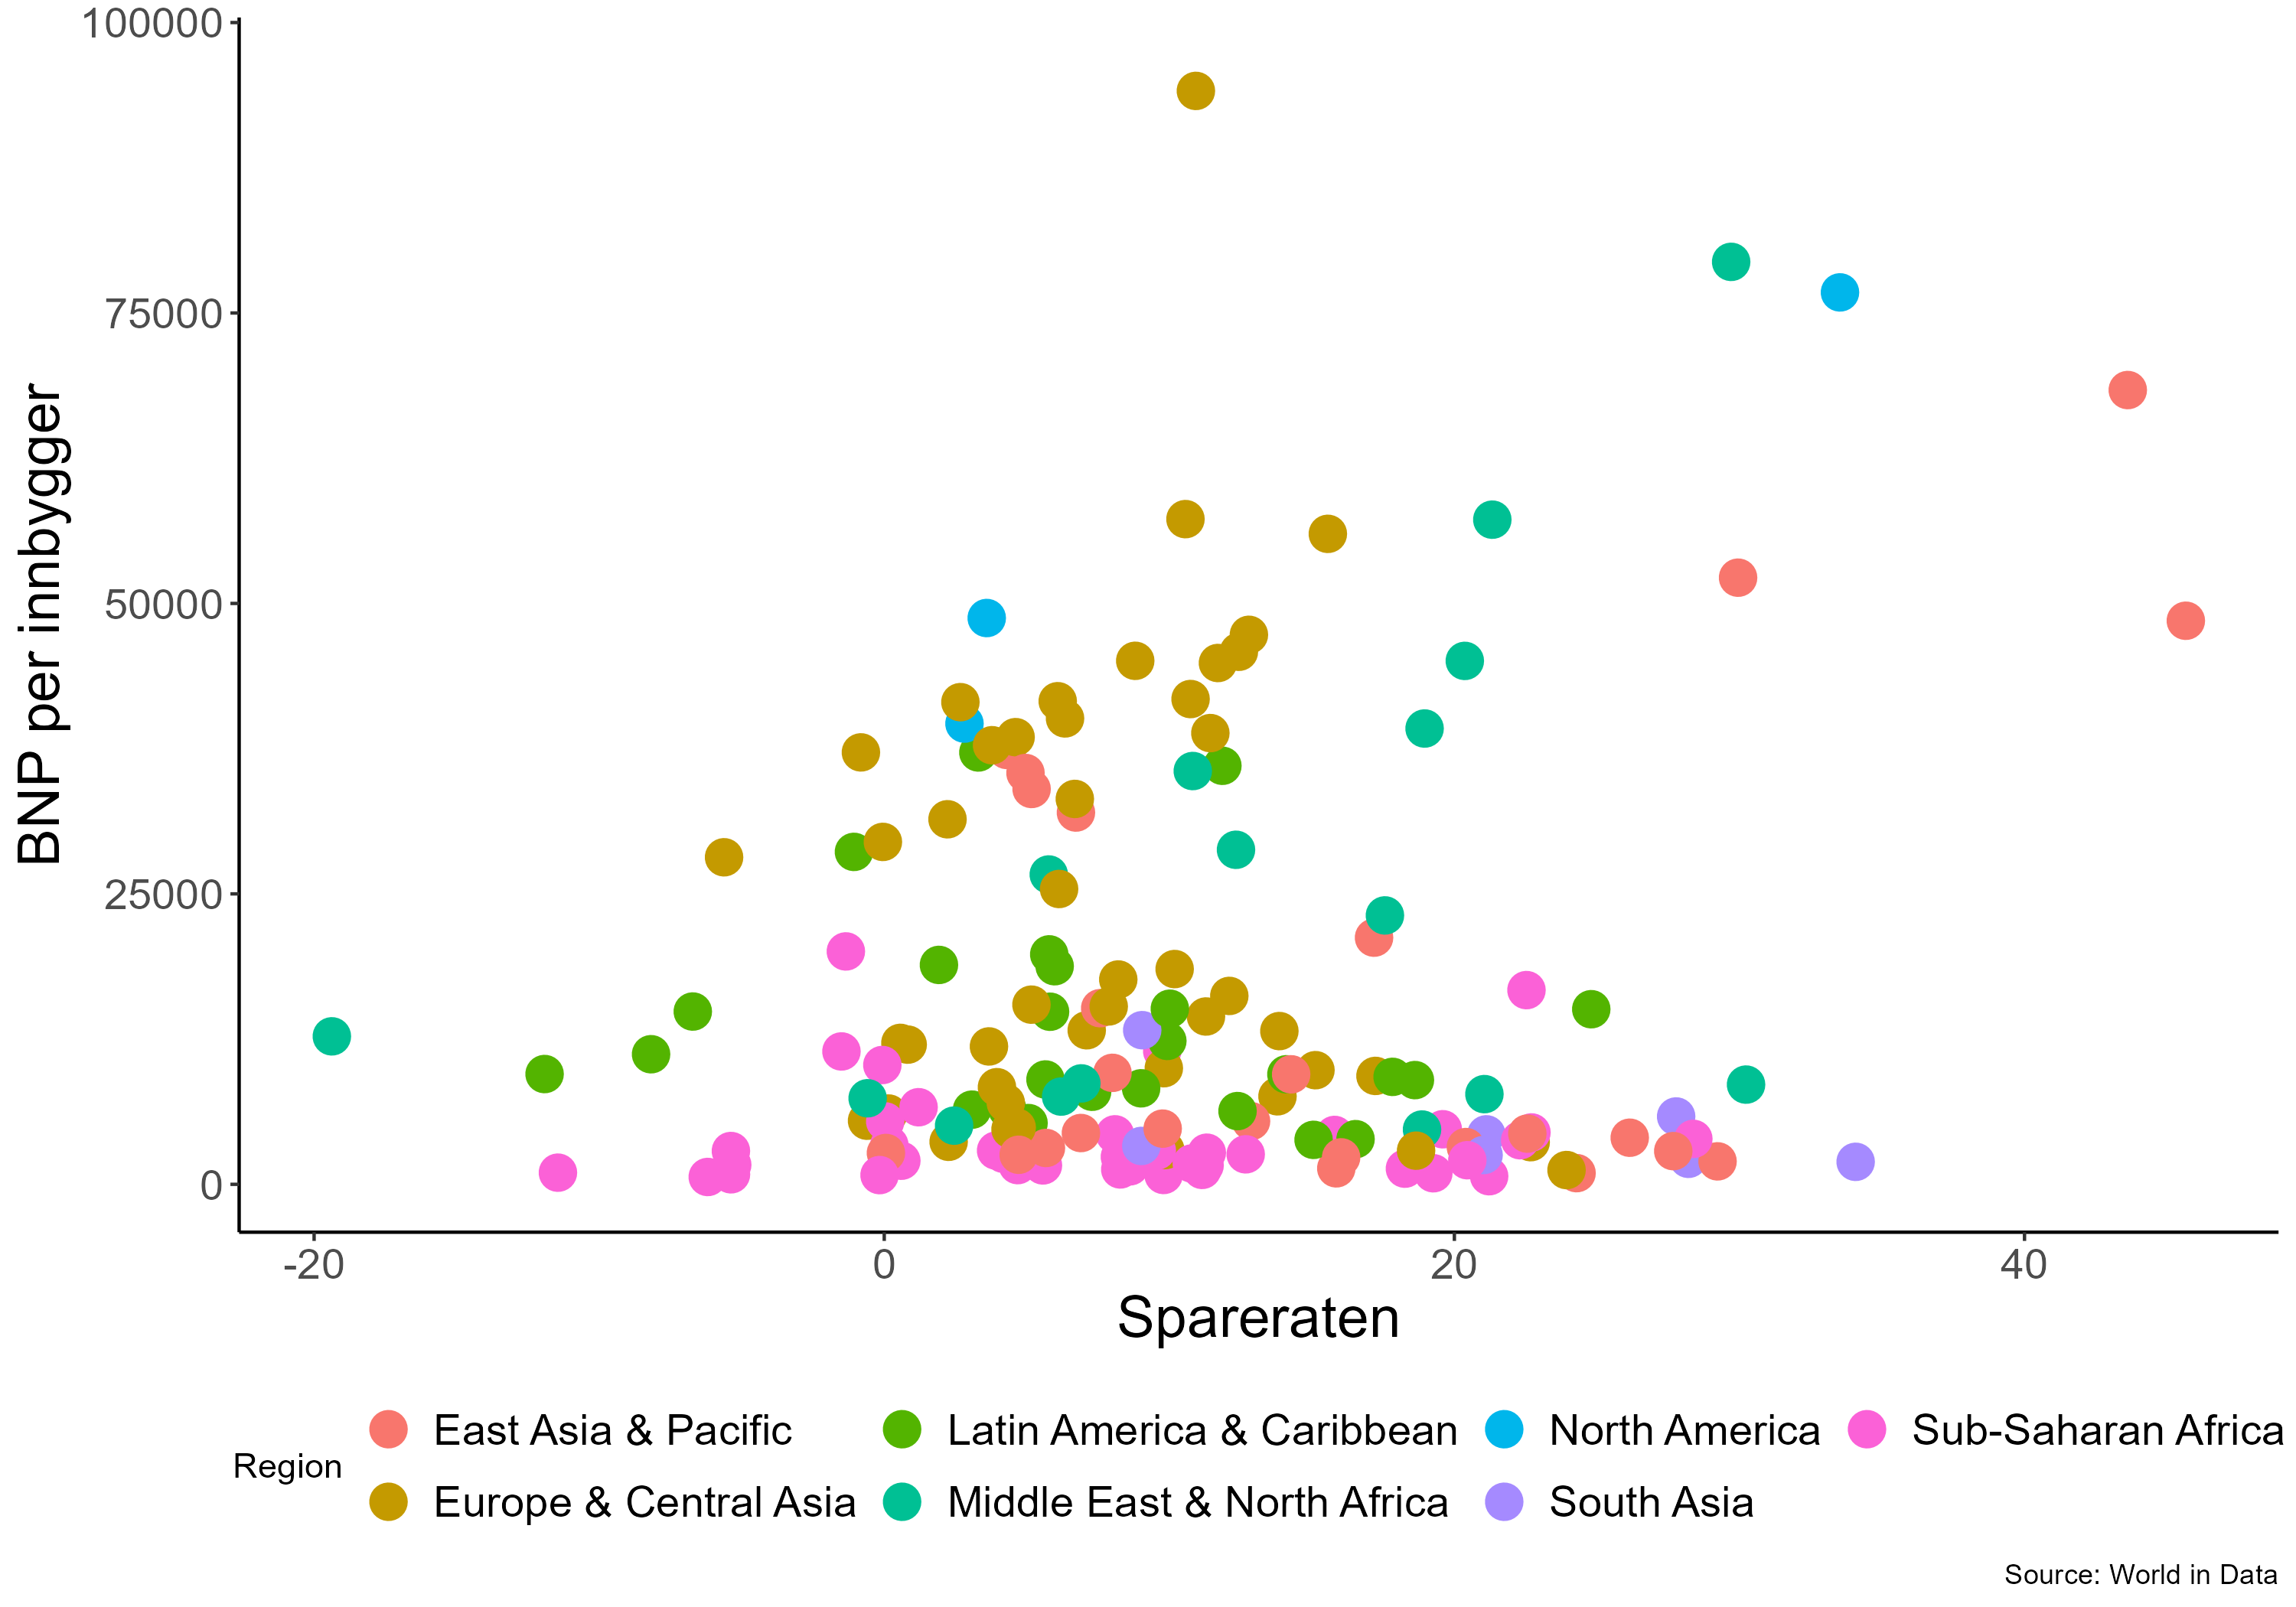
\includegraphics[width=0.5\textwidth]{dokumentobjekter/figurer/spareraten_bnp_per_innbygger.png}
  \captionof{figure}{Sparerate}
  \label{fig:sparerate}
  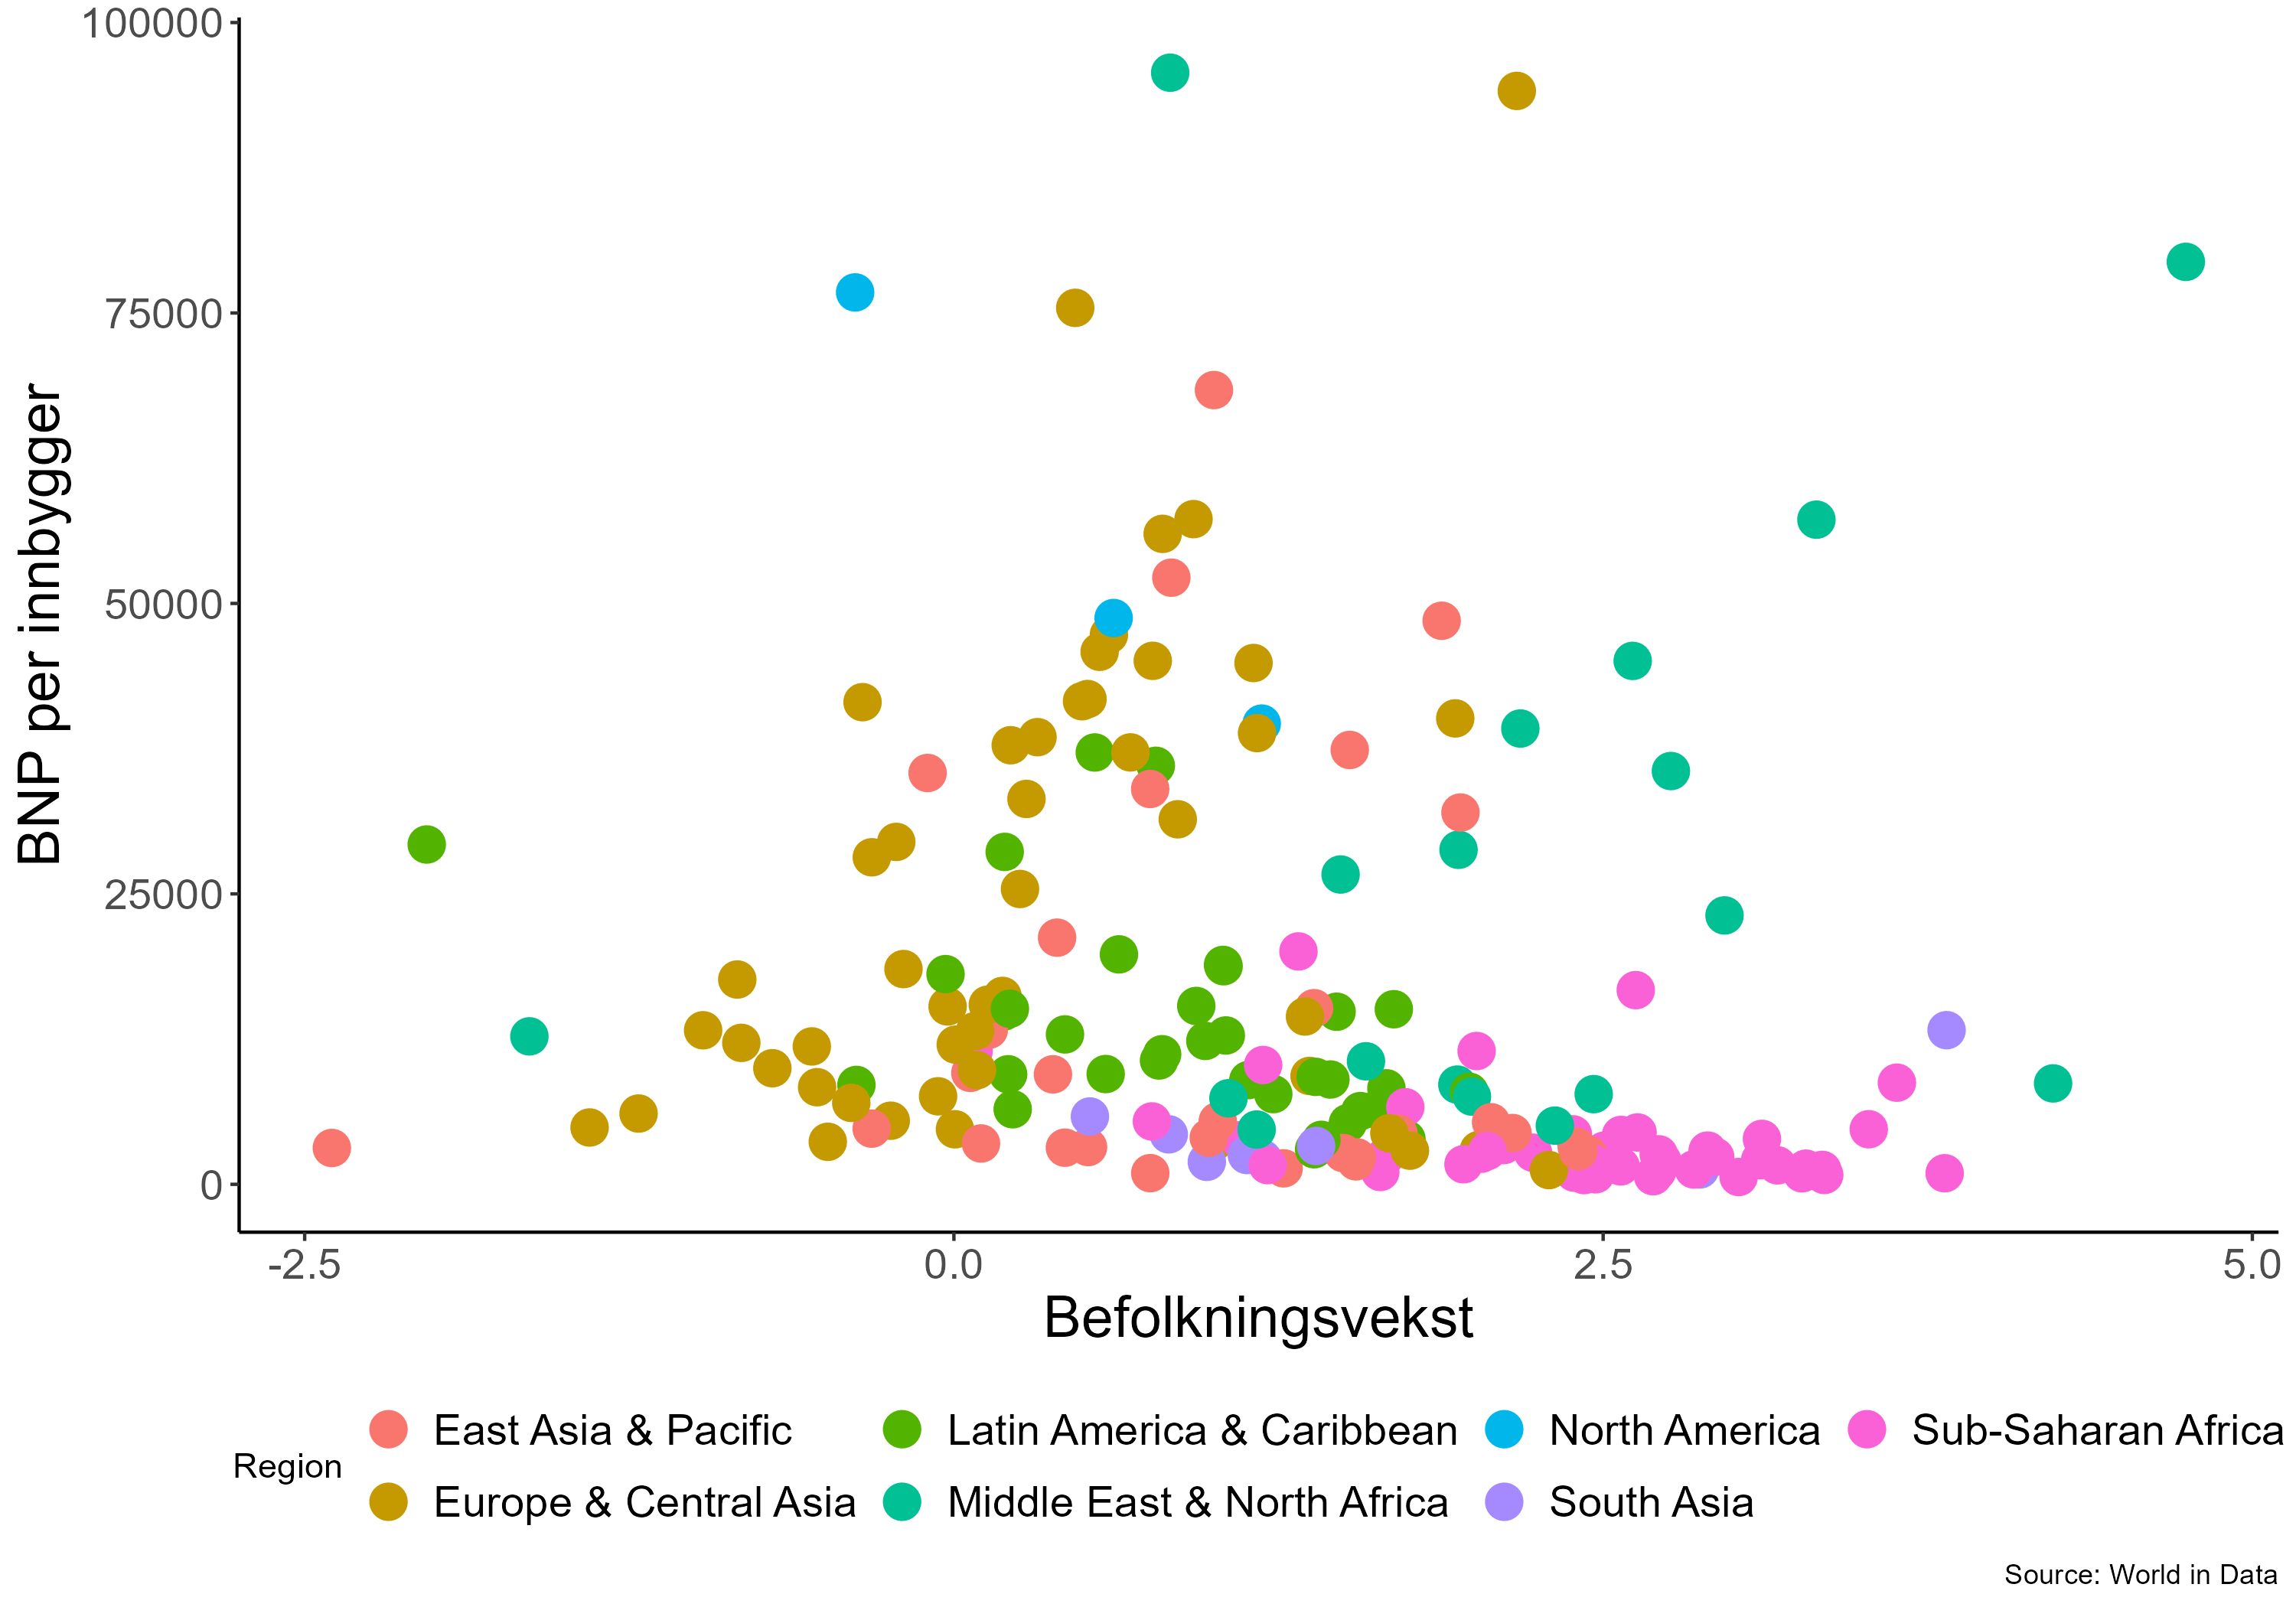
\includegraphics[width=0.5\textwidth]{dokumentobjekter/figurer/befolkningsvekst_bnp_per_innbygger.png}
  \captionof{figure}{Befolkningsvekst}
  \label{fig:befolkningsvekst}
  \vspace{-10mm}
\end{wrapfigure}

I \autoref{fig:sparerate} ser vi at det er en svak positiv sammenheng
mellom spareraten og BNP per innbygger. Dette betyr at land med høyere
sparerate har høyere BNP per innbygger. Dette er i tråd med
prediksjonene fra Solow-modellen, som sier at økt sparing fører til økt
investering, som igjen fører til økt kapital og økt produksjon.

I \autoref{fig:befolkningsvekst} ser vi at det er en svak negativ
sammenheng mellom befolkningsvekst og BNP per innbygger. Dette betyr at
land med høyere befolkningsvekst har lavere BNP per innbygger. Dette er
også i tråd med prediksjonene fra Solow-modellen, som sier at økt
befolkningsvekst fører til lavere BNP per innbygger, fordi det blir
flere mennesker som skal dele på investeringene. Hvis befolkningen
vokser raskere, så trenges det mer kapital per arbeider, som gjør at
produksjon per arbeider går ned.\footnote{Sitat hentet fra utfordring 1
  i SOK-2011 fra kandidatnummer 70, 84, 72}

Det er svake sammenhenger vi kan observere i figurene så derfor
estimerer vi en OLS (minste kvadrats-metode) som tester om spareraten og
befolkningsveksten forklarer variasjon i BNP per innbygger mellom ulike
land.

\clearpage

\subsubsection{b. Estimer en regresjonsmodell (minste kvadrats-metode)
som tester om spareraten og befolkningsveksten forklarer variasjon i BNP
per innbygger mellom ulike
land.}\label{b.-estimer-en-regresjonsmodell-minste-kvadrats-metode-som-tester-om-spareraten-og-befolkningsveksten-forklarer-variasjon-i-bnp-per-innbygger-mellom-ulike-land.}

Hvorfor kjører vi en regresjonsanalyse? Regresjonsanalyse hjelper oss
med å forstå hvordan ulike variabler henger sammen. Den brukes til å
forutsi verdier av en avhengig variabel basert på en eller flere
uavhengige variabler. Den er effektiv til å analysere store datamengder
for å finne trender og mønstre som kanskje ikke er tydelige ved første
øyekast.

Modellen vårs skal teste om BNP per innbygger kan forklares av
spareraten og befolkningsveksten. Modellen er som følger:

\[ y_{i,2015-2019} = \alpha_y + \beta_1 \cdot s_{i,2010-2015} + \beta_2 \cdot n_{i,2010-2015} + \epsilon_i \]

Hvor \(y_{i,2015-2019}\) er BNP per innbygger i land \(i\) i perioden
2015-2019, \(s_{i,2010-2015}\) er spareraten i land \(i\) i perioden
2010-2015, \(n_{i,2010-2015}\) er befolkningsveksten i land \(i\) i
perioden 2010-2015, \(\alpha_y\) er en konstant, \(\beta_1\) og
\(\beta_2\) er koeffisienter som forteller oss hvor mye BNP per
innbygger endrer seg når spareraten og befolkningsveksten endrer seg, og
\(\epsilon_i\) er et feilledd.

\begin{table}[!htbp] \centering 
  \caption{Regresjonsmodel sparerate og befolkningsvekst påvirkning på bnp} 
  \label{tab:table1} 
\begin{tabular}{@{\extracolsep{5pt}}lc} 
\\[-1.8ex]\hline 
\hline \\[-1.8ex] 
 & \multicolumn{1}{c}{Avhengig variabel} \\ 
\cline{2-2} 
\\[-1.8ex] & BNP per innbygger \\ 
\hline \\[-1.8ex] 
 Sparerate & 570.892$^{***}$ \\ 
  & (172.252) \\ 
  & \\ 
 Befolkningsvekst & $-$4,255.577$^{***}$ \\ 
  & (1,419.727) \\ 
  & \\ 
 Constant & 21,623.470$^{***}$ \\ 
  & (2,789.207) \\ 
  & \\ 
\hline \\[-1.8ex] 
Observations & 165 \\ 
R$^{2}$ & 0.090 \\ 
Adjusted R$^{2}$ & 0.079 \\ 
Residual Std. Error & 21,684.770 (df = 162) \\ 
F Statistic & 8.037$^{***}$ (df = 2; 162) \\ 
\hline 
\hline \\[-1.8ex] 
\textit{Note:}  & \multicolumn{1}{r}{$^{*}$p$<$0.1; $^{**}$p$<$0.05; $^{***}$p$<$0.01} \\ 
\end{tabular} 
\end{table}

På neste side tolker vi resultatene fra regresjonsanalysen.

\clearpage

\subsubsection{c.~Tolke resultatene fra spredningsdiagrammen og
regresjonsanalysen.}\label{c.-tolke-resultatene-fra-spredningsdiagrammen-og-regresjonsanalysen.}

Constanten eller \(\alpha_y\) i regresjonsanalysen er 21623.47. Dette
betyr at hvis spareraten og befolkningsveksten er 0, så vil BNP per
innbygger være 21623.47. Dette tallet gir oss en pekepinn på hvor mye
BNP per innbygger ville vært hvis spareraten og befolkningsveksten var
0.

Koeffisienten til spareraten eller \(\beta_1\) er positiv. Dette betyr
at hvis spareraten øker så vil BNP per innbygger øke. Dette er i tråd
med prediksjonene fra Solow-modellen og *** sier at resultatet er
signifikant og ikke har oppstått ved tilfeldighet (p \textless{} 0.05).

Koeffisienten til befolkningsveksten eller \(\beta_2\) er negativ. Dette
betyr at hvis befolkningsveksten øker, så vil BNP per innbygger gå ned.
Dette er også i tråd med prediksjonene fra Solow-modellen og *** sier at
resultatet er signifikant og ikke har oppstått ved tilfeldighet (p
\textless{} 0.05) her også, dette blir forklart bedre hvordan fungerer i
\hyperref[c.-tolke-resultatene-fra-spredningsdiagrammene-og-regresjonsanalysen-og-diskutere-eventuelle-svakheter-eller-begrensninger.]{del 2.3}.

Degrees of freedom (observations) er antall uavhengige observasjoner i
datasettet minus antall parametere som estimeres i modellen. I dette
tilfellet er observations 165, som betyr at det er 165 uavhengige
observasjoner i datasettet, noe som da er antall land som er med i
datasettet.

Residual standard error er et mål på hvor mye de avhengige variablene
varierer rundt den estimerte regresjonslinjen. I dette tilfellet er
residual standard error 21684.7, som betyr at de avhengige variablene
varierer rundt den estimerte regresjonslinjen med 21684.7 enheter, som
kan være en svakhet med modellen.

\(R^2\) er et mål på hvor mye variasjon i den avhengige variabelen som
forklares av de uavhengige variablene. I dette tilfellet er \(R^2\)
0.079, som betyr at omtrent 8\% av variasjonen i BNP per innbygger kan
forklares av spareraten og befolkningsveksten. Dette er et relativt høyt
tall for BNP per innbygger, selv om det er mye av variansen som ikke kan
forklares av modellen.

Totalt sett så er resultatene fra regresjonsanalysen i tråd med de små
sammenhengene man kan se fra \autoref{fig:sparerate} og
\autoref{fig:befolkningsvekst} og likt som hva Solow-modellen predikerer
og viser at spareraten og befolkningsveksten kan forklare variasjon i
BNP per innbygger mellom ulike land.

\clearpage

\subsection{Utfordring 2.3}\label{utfordring-2.3}

\subsubsection{a. Spredningsdiagram som viser sammenhengen mellom
Humankapital, forbruket av naturressurser og og initialt nivå på BNP per
innbygger mot vekstraten i BNP per
innbygger.}\label{a.-spredningsdiagram-som-viser-sammenhengen-mellom-humankapital-forbruket-av-naturressurser-og-og-initialt-nivuxe5-puxe5-bnp-per-innbygger-mot-vekstraten-i-bnp-per-innbygger.}

\begin{wrapfigure}{r}{0.5\textwidth}
  \centering
  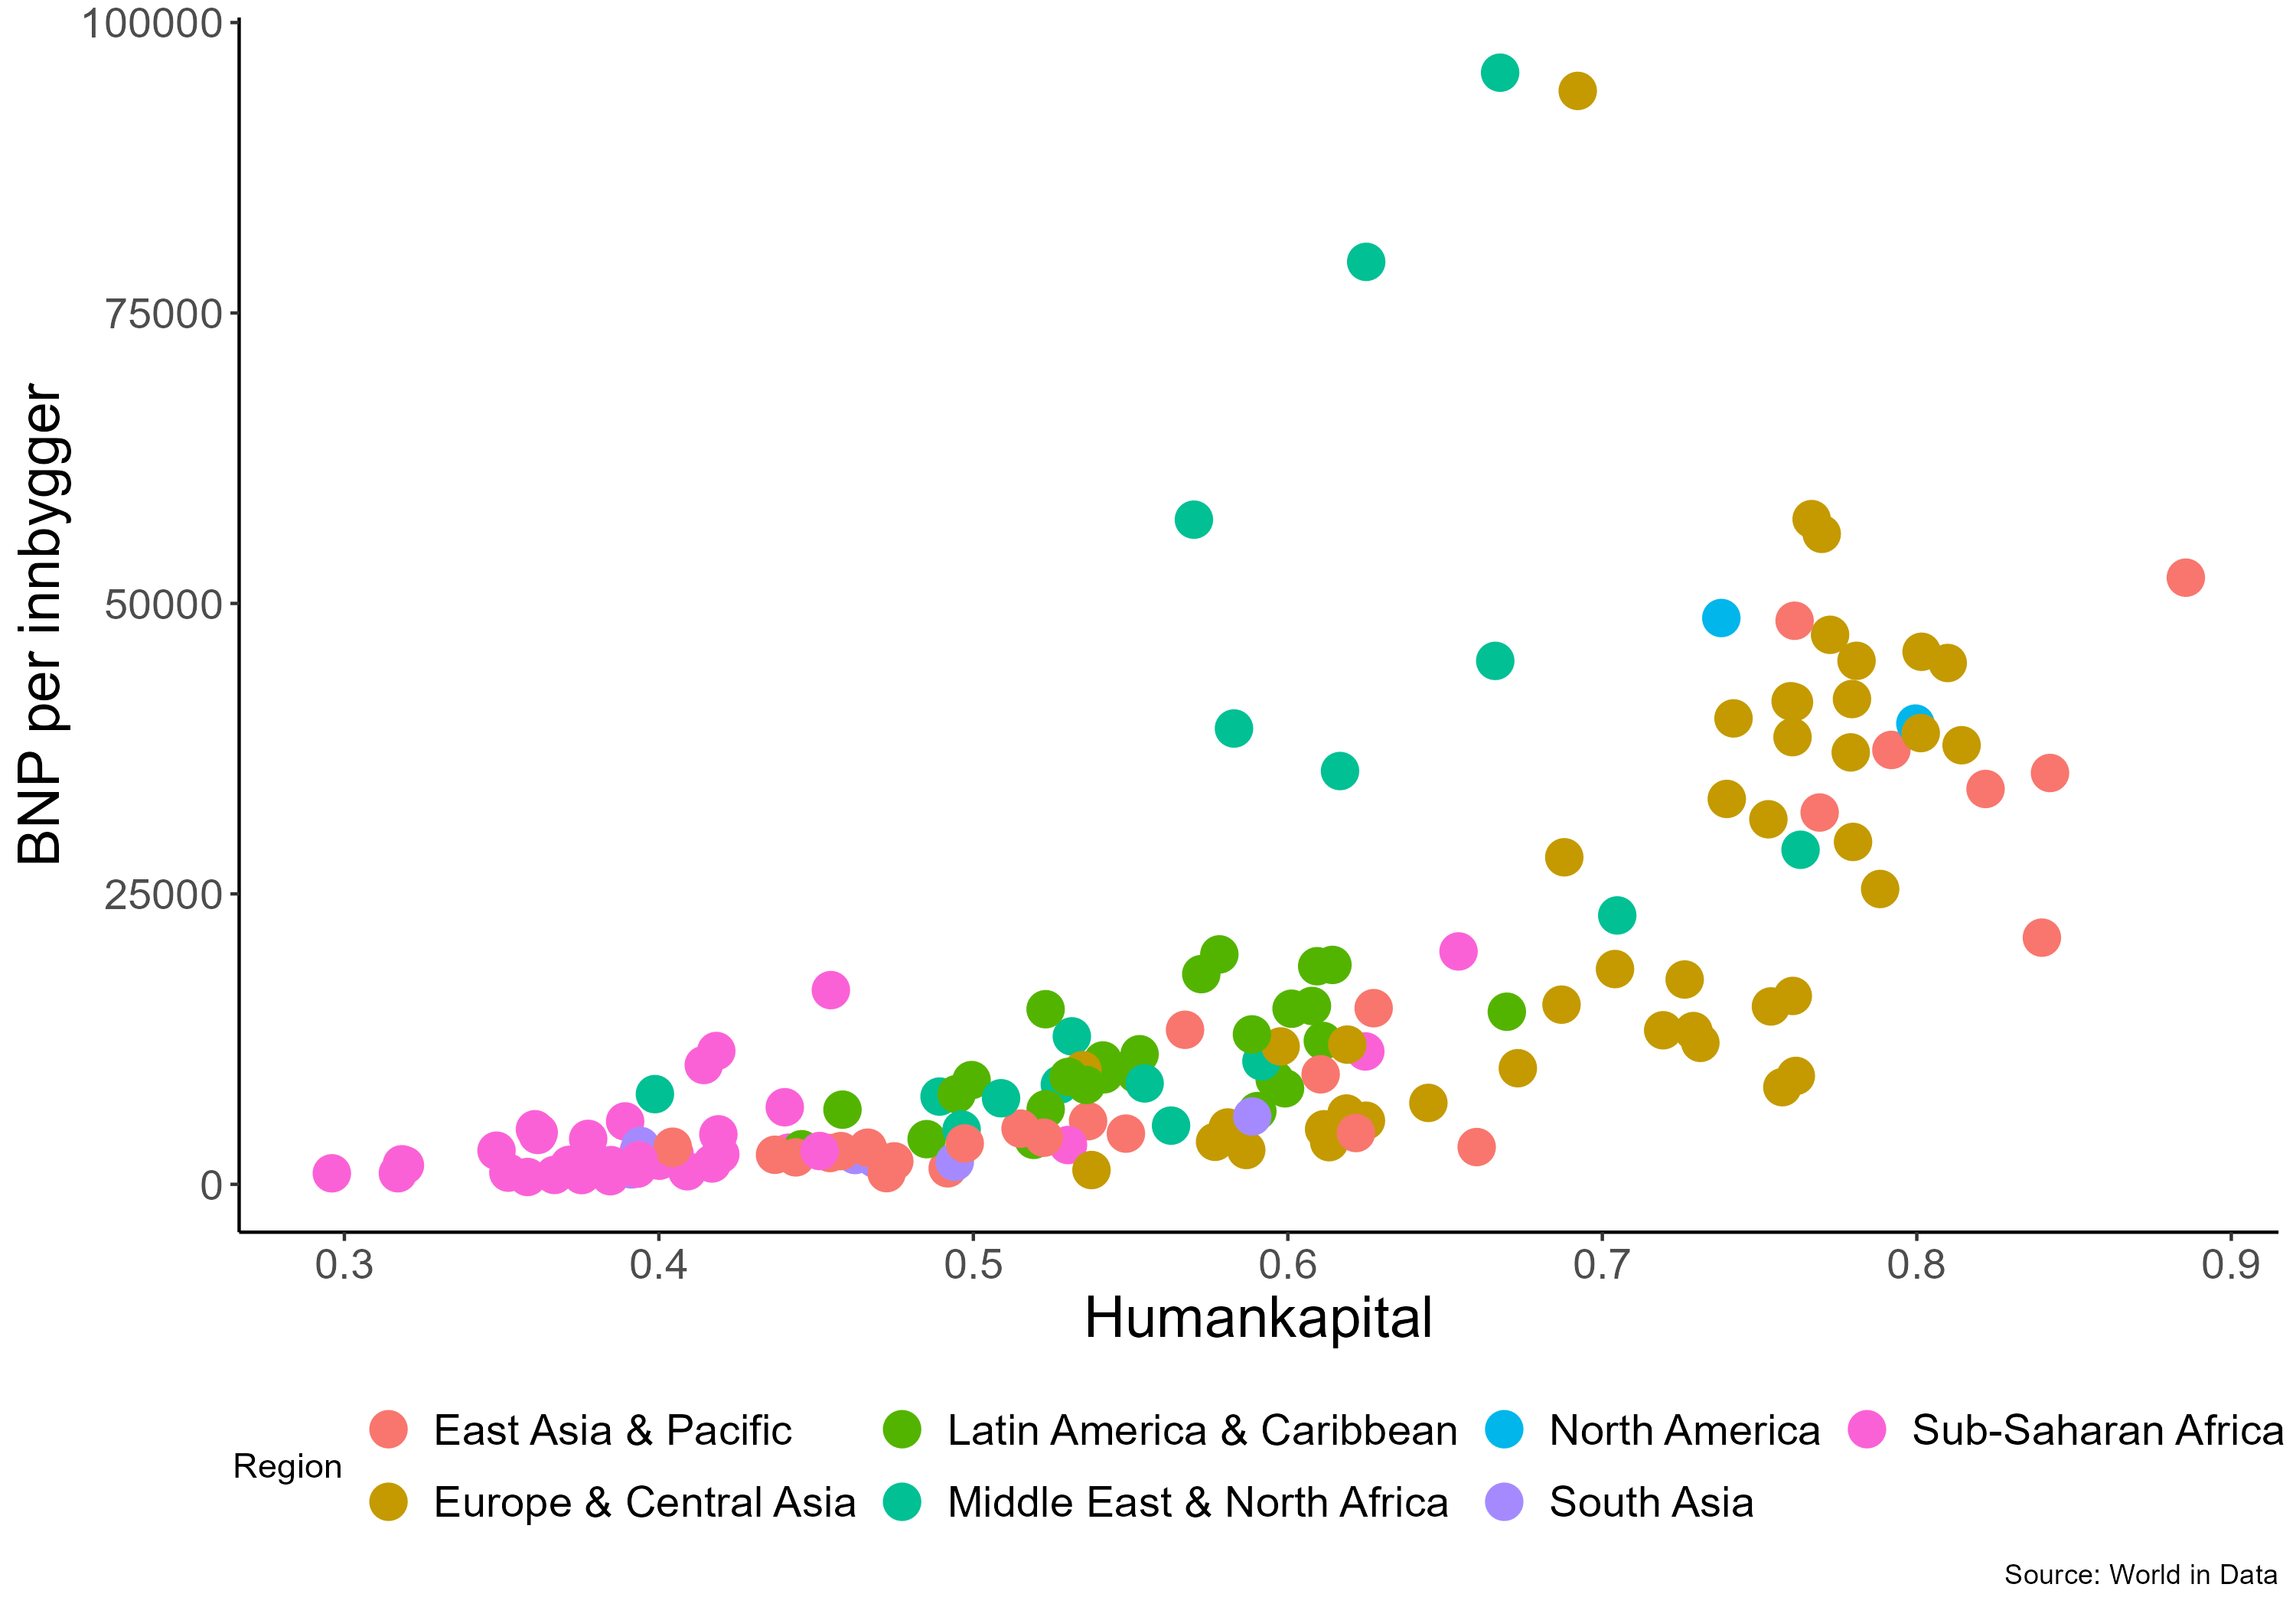
\includegraphics[width=0.5\textwidth]{dokumentobjekter/figurer/humankapital_bnp_per_innbygger.png}
  \captionof{figure}{Humankapital}
  \label{fig:humankapital}
  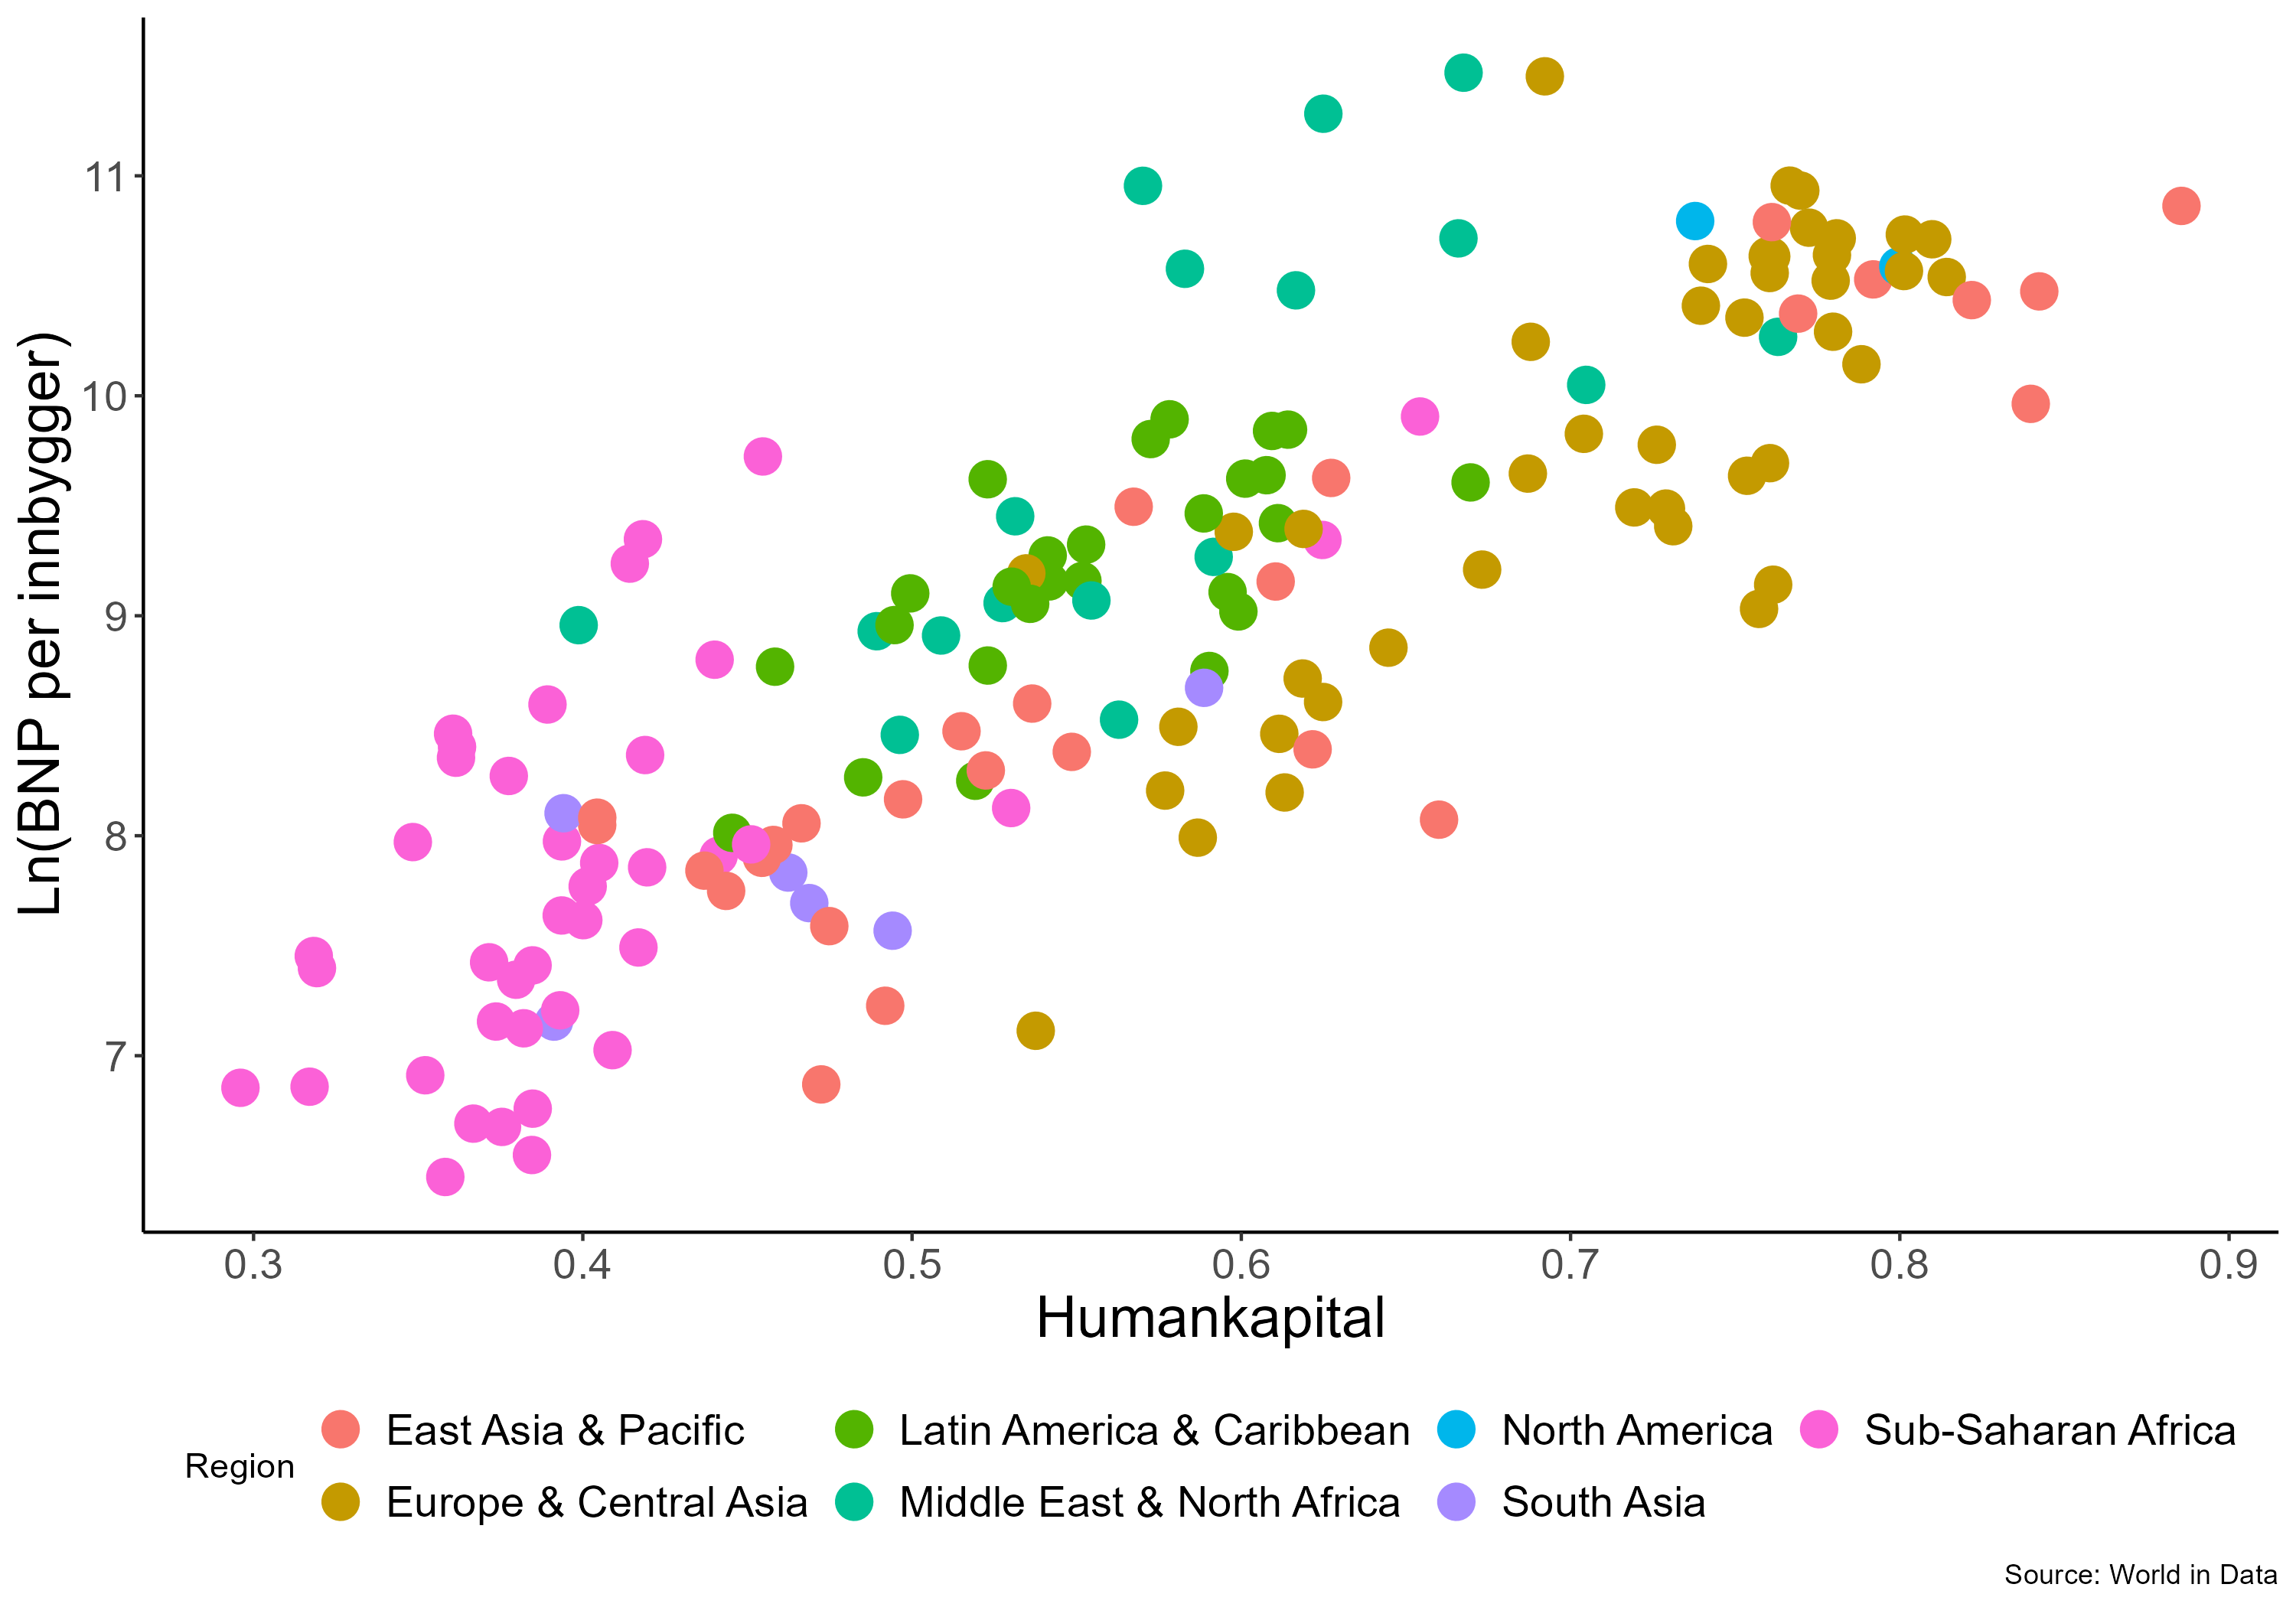
\includegraphics[width=0.5\textwidth]{dokumentobjekter/figurer/humankapital_bnp_per_innbygger_log.png}
  \captionof{figure}{Humankapital logaritmisk BNP per innbygger}
  \label{fig:humankapital_log}
    \vspace{-8mm}
\end{wrapfigure}

I motsetning til figurer i
\hyperref[c.-tolke-resultatene-fra-spredningsdiagrammen-og-regresjonsanalysen.]{del 2.2}
så kan vi i \autoref{fig:humankapital} se at humankapital har en
påvirkning på BNP per innbygger. I Europa og Sentral-Asia ser vi
spesielt en vekst i BNP når humankapital øker, mens vi ser at Afrika sør
for Sahara har en lavere BNP per innbygger og lavere humankapital. Dette
er i tråd med Solow-modellen, som sier at humankapital er en viktig
faktor for økonomisk vekst, men i motsetning til Utfordring 1, så ser
det ikke ut til å være en lineær sammenheng mellom humankapital og BNP
per innbygger.

Dersom vi tar humankapital i mot logaritmen til BNP per innbygger vist i
\autoref{fig:humankapital_log} så kan vi se et langt mye tydeligere
bilde av sammenhengen mellom humankapital og BNP per innbygger. Vi ser
at det er en positiv sammenheng mellom humankapital og BNP per innbygger
i alle regioner i verden. Dette er i tråd med Solow-modellen. Når vi
gjør lineær regresjonsanalyse så blir vi å bruke logaritmen av bnp per
innbygger siden uten logaritmen så er det en sammenheng men den er ikke
lineær.

\clearpage

\begin{wrapfigure}{h}{0.5\textwidth}
  \centering
  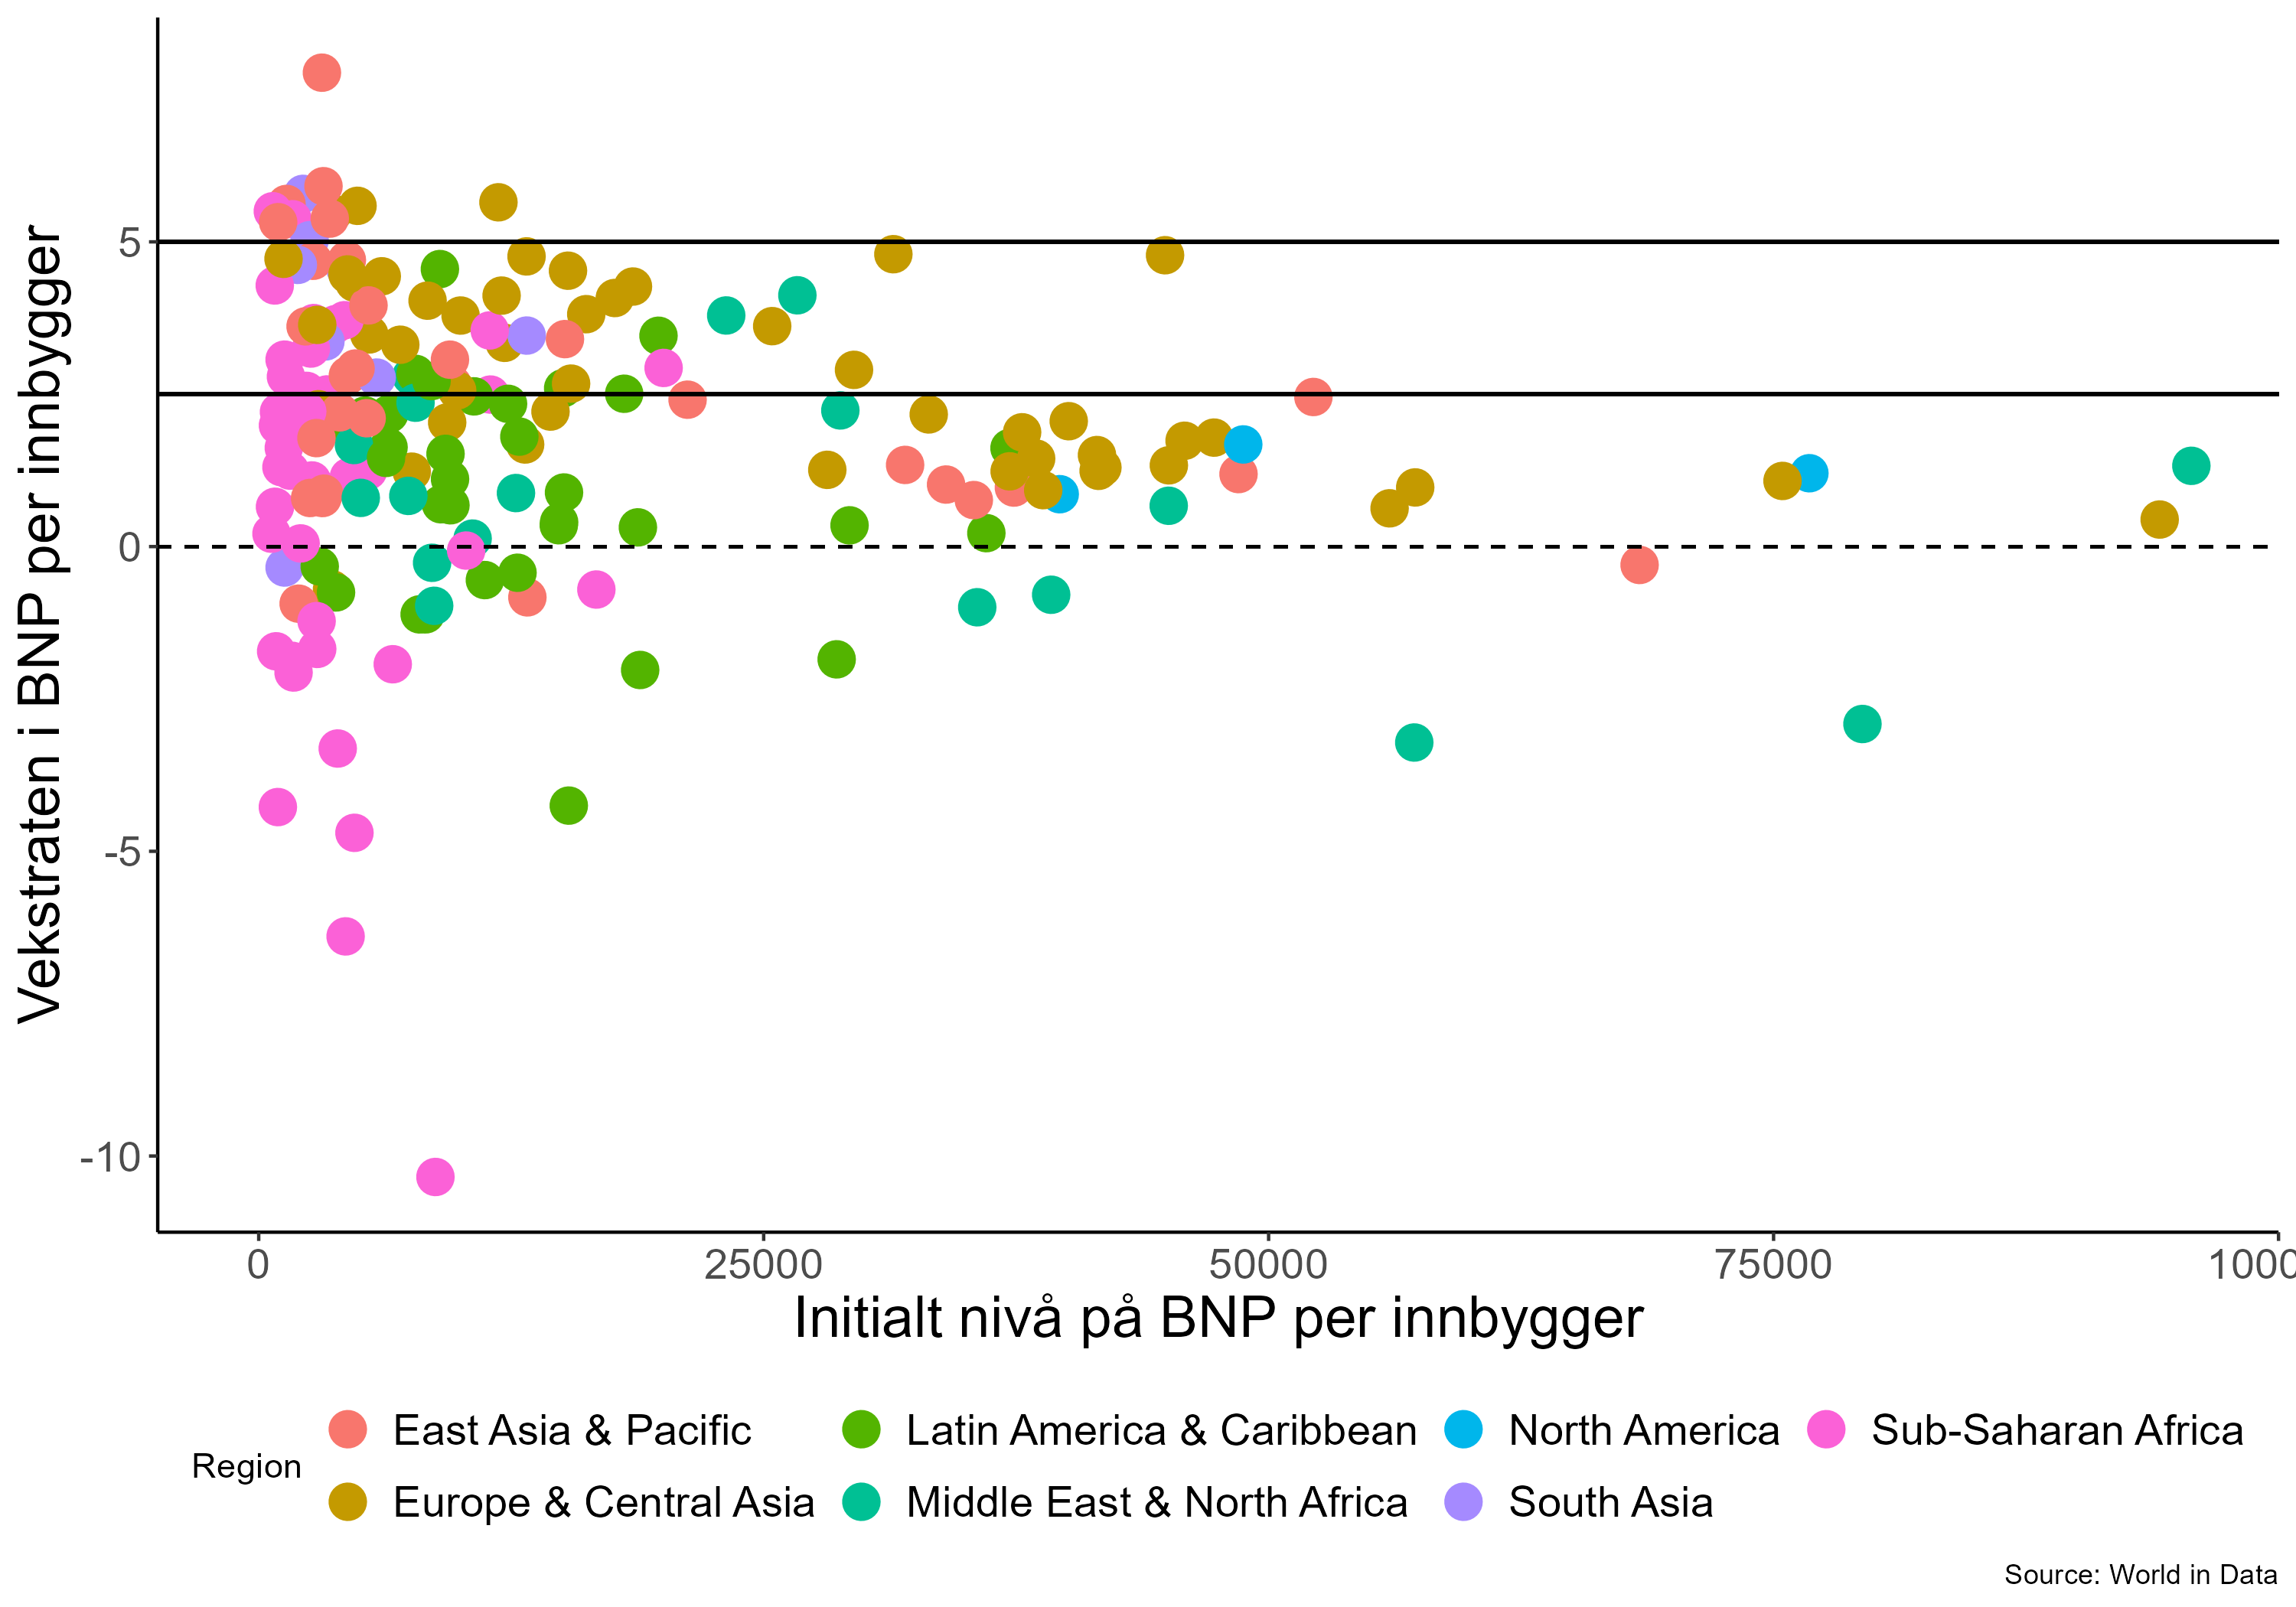
\includegraphics[width=0.5\textwidth]{dokumentobjekter/figurer/vekstrate_bnp_per_innbygger.png}
  \captionof{figure}{Vekstrate i BNP per innbygger}
  \label{fig:vekstrate}
  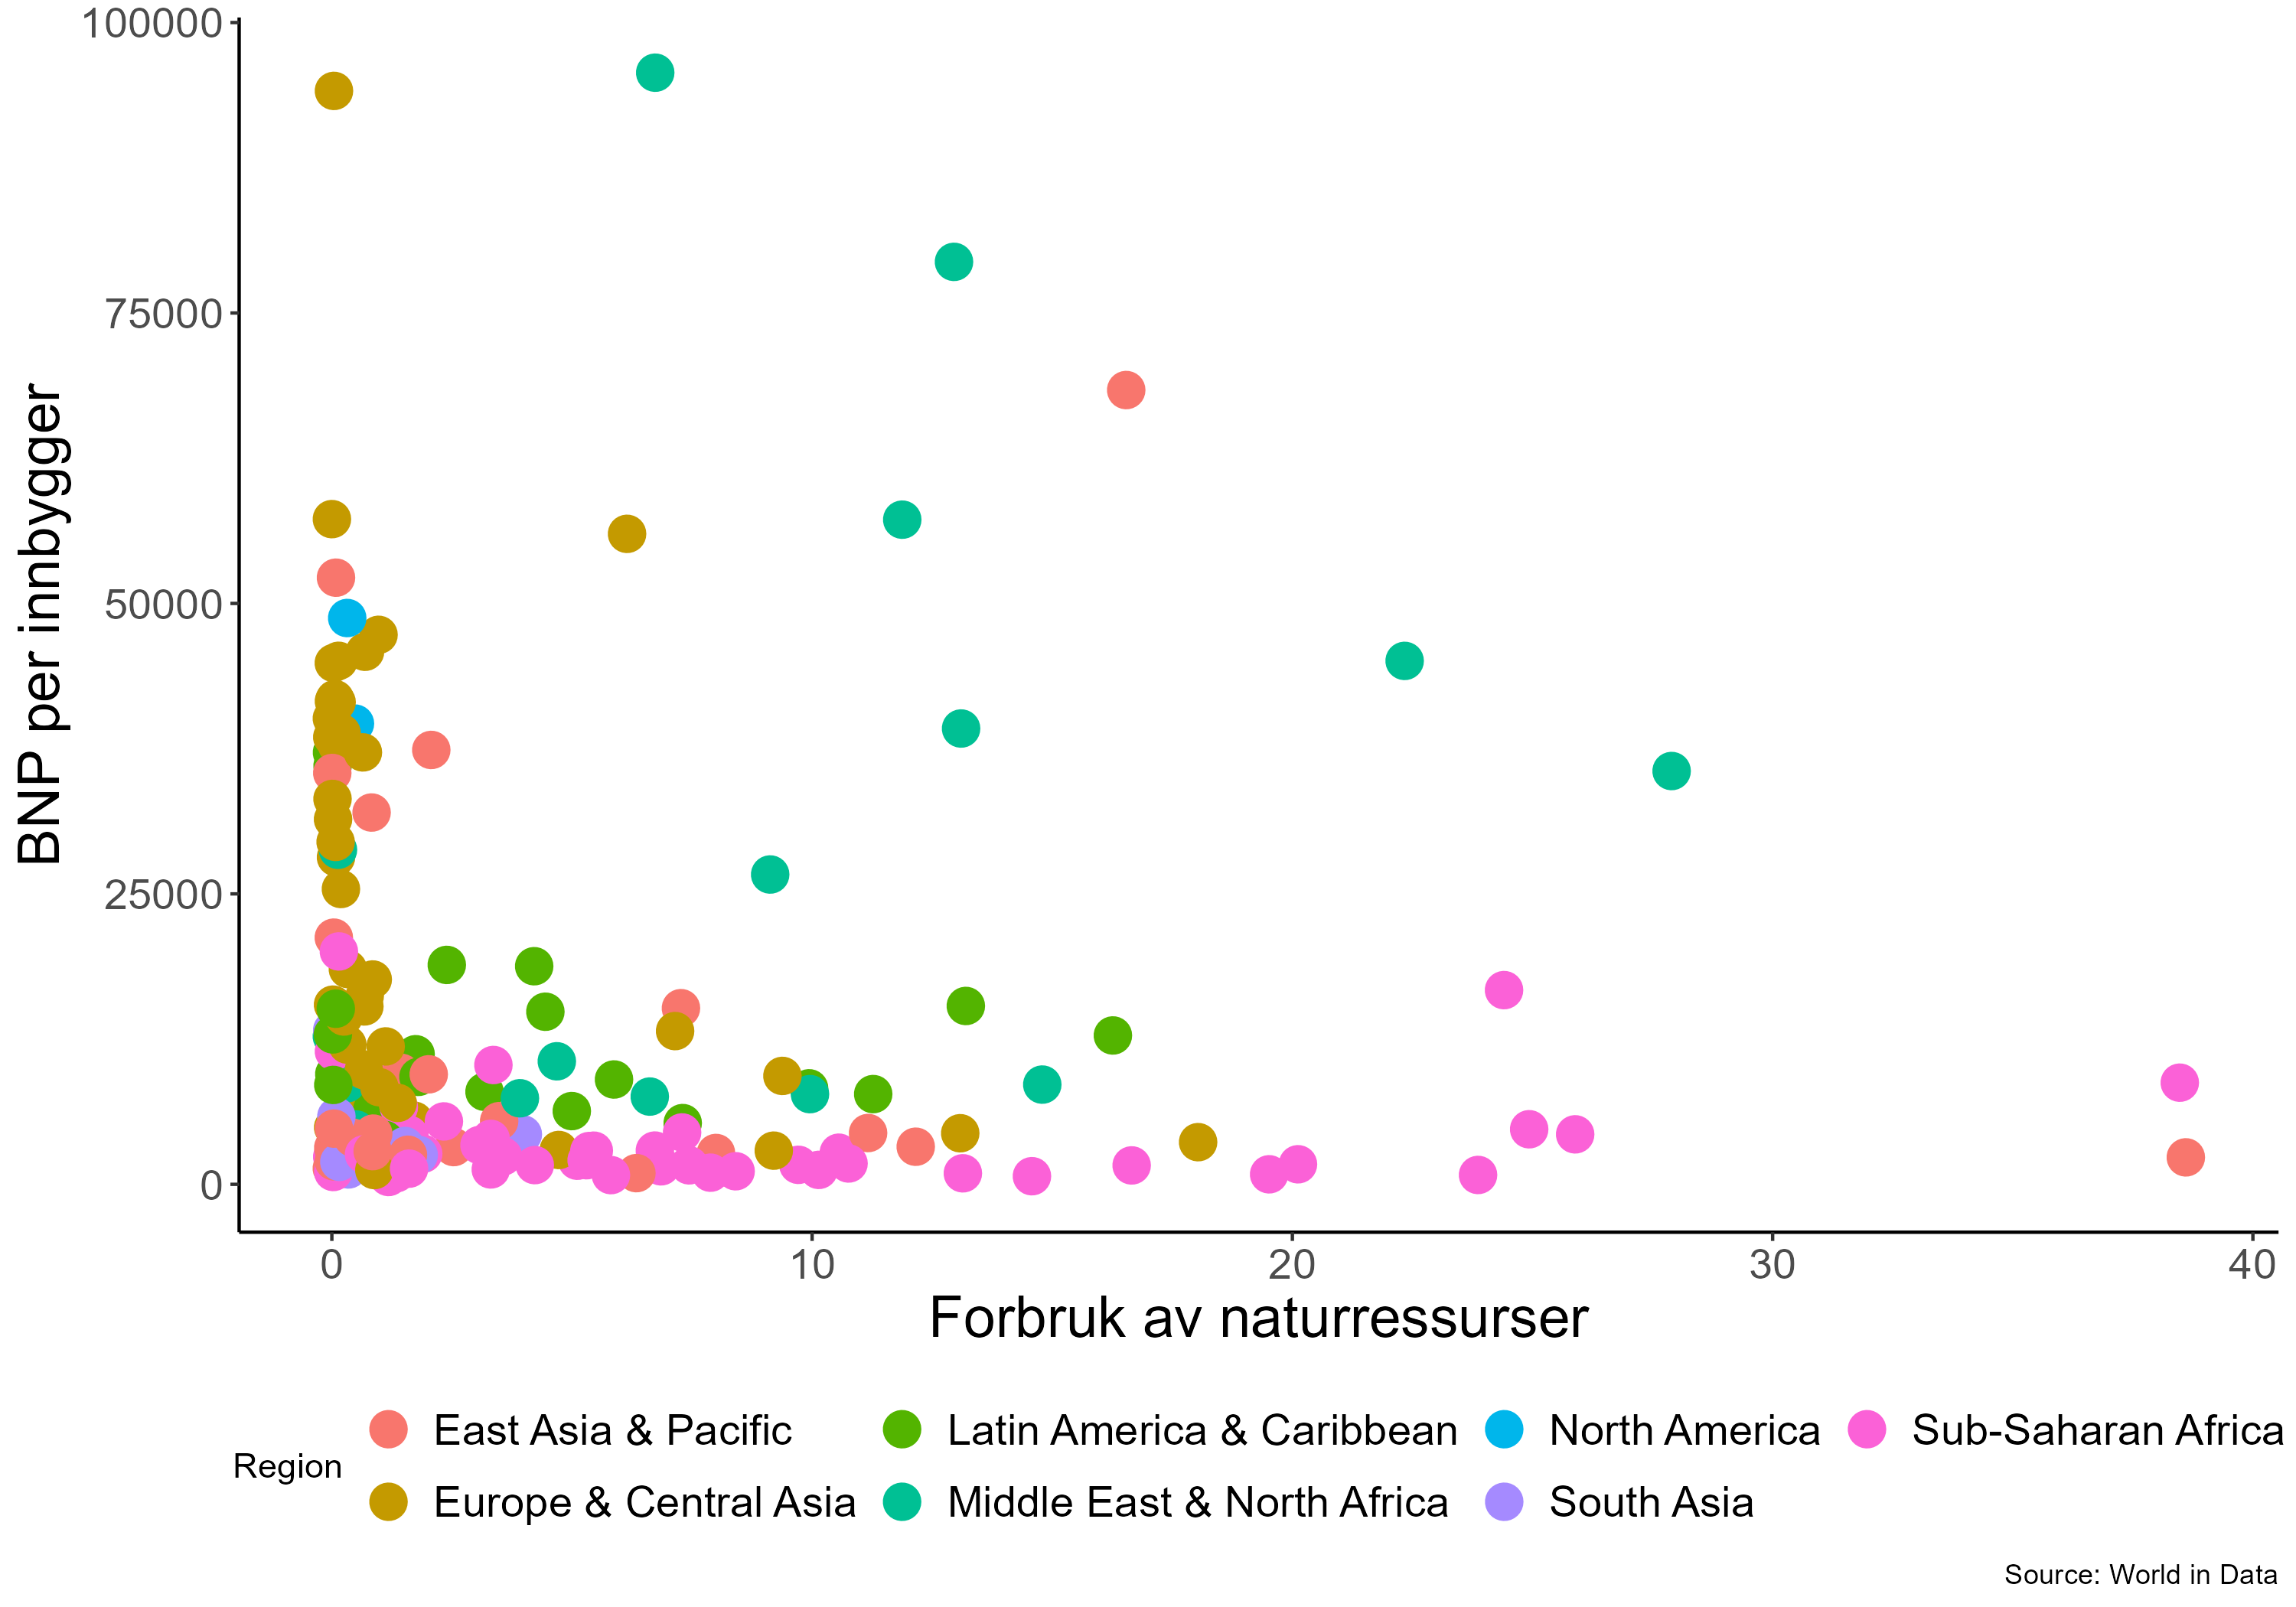
\includegraphics[width=0.5\textwidth]{dokumentobjekter/figurer/naturressurser_bnp_per_innbygger.png}
  \captionof{figure}{Naturressurser}
  \label{fig:naturressurser}
  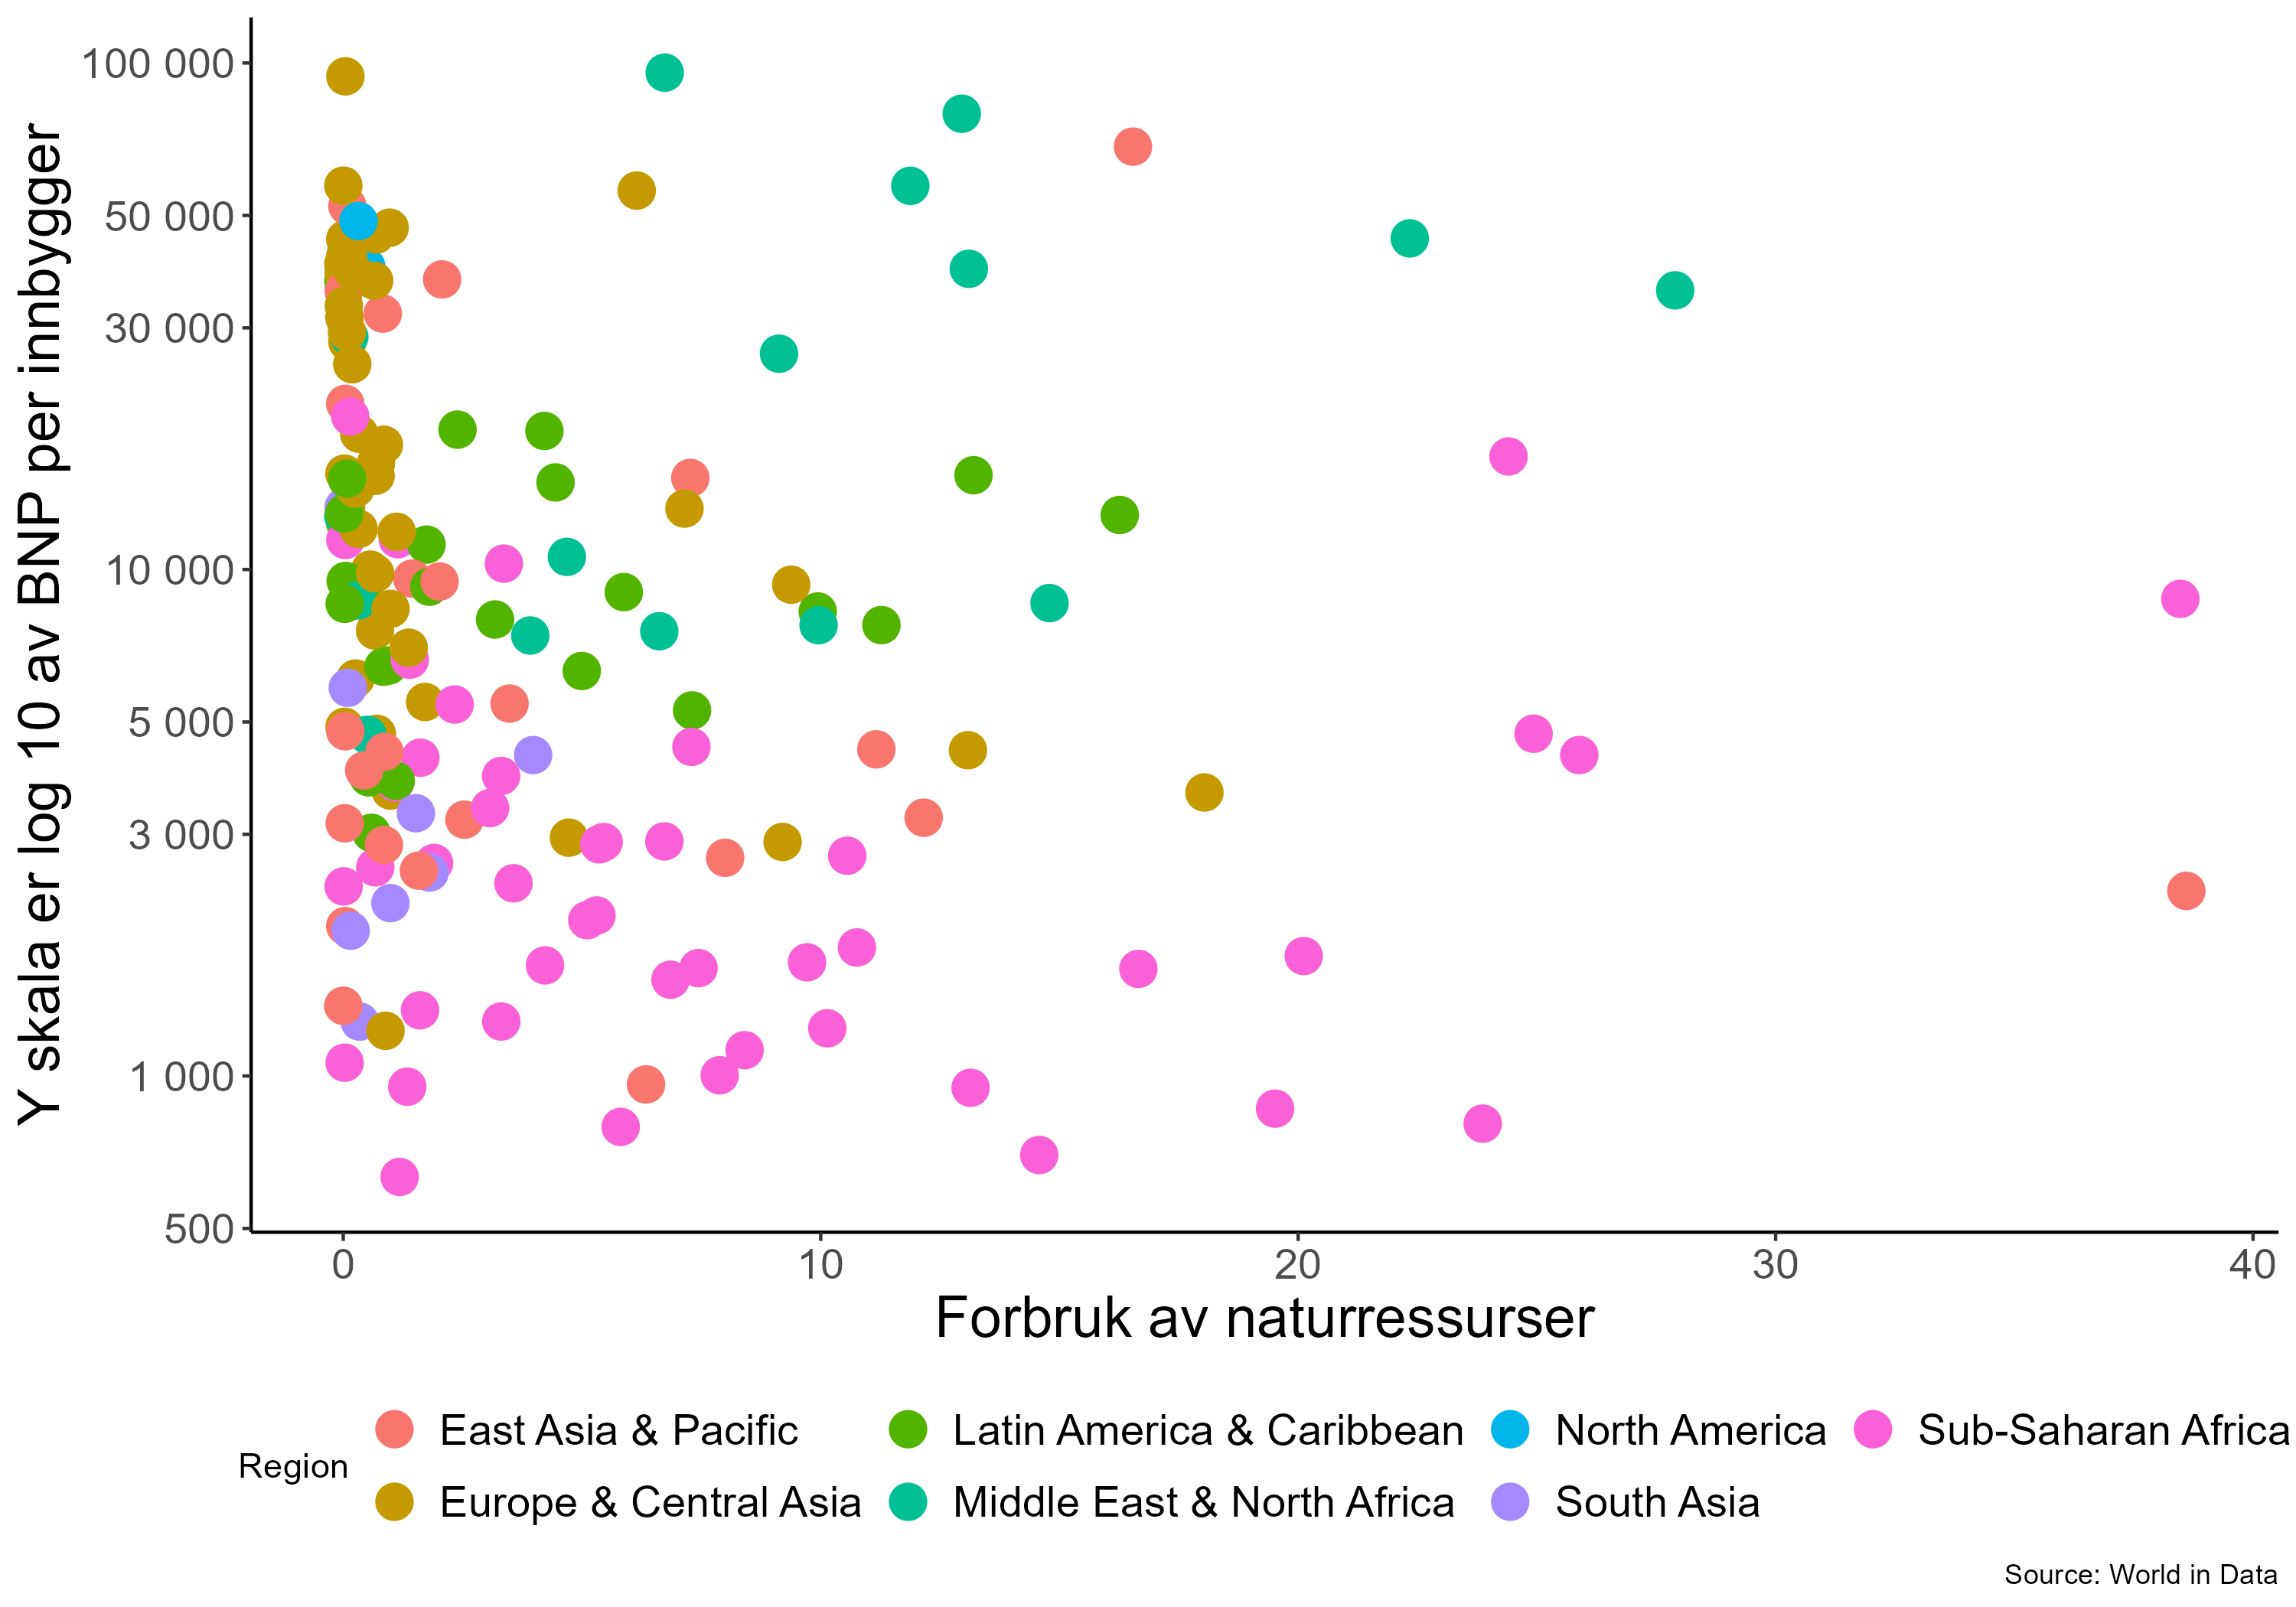
\includegraphics[width=0.5\textwidth]{dokumentobjekter/figurer/naturressurser_bnp_per_innbygger_log.png}
  \captionof{figure}{Naturressurser med log y-akse}
  \label{fig:naturressurser_log}
  % \vspace{-8mm}
\end{wrapfigure}

I \autoref{fig:vekstrate} ser vi effekten det initielle nivået på BNP i
perioden hadde på vekstraten i BNP per innbygger. Det er tegnet inn en
striplet linje på 0\% vekst, med solide linjer på 2.5\% og på 5\%. Her
ser vi at det er veldig få land som har en veldig høy BNP per innbygger
som også har en høy vekstrate, men de fleste som har den høye vekstraten
har et lavt initialt nivå på BNP per innbygger.

\autoref{fig:naturressurser} viser forbruk av naturressurser sin effekt
på i BNP per innbygger. Her er det noe vanskeligere å se noe lineær
sammenheng, men det ser ut til at land som har et høyt forbruk av
naturressurser har en lavere BNP per innbygger hvor vi kan se en samling
langs x-aksen. Langs y aksen nær 0 forbruk i naturressurser ser vi en
gruppering av land med høy BNP per innbygger. Denne L formen vi får på
figuren kan fortelle oss at det er en negativ sammenheng mellom forbruk
av naturressurser og BNP per innbygger.

Ved å ta å skalere y aksen med \(log_{10}\) i
\autoref{fig:naturressurser_log} så blir det en noe tydeligere
sammenheng men \textbf{merk} at det er en annen skala på y aksen i denne
figuren. Det vi nå kan se er at de fleste landene som har under 10000 i
BNP per innbygger har et høyere forbruk av naturressurser. Vi ser også
at dette i stor grad er afrikanske land der det kan være andre faktorer
som spiller inn som foresaker deres lavere BNP per innbygger. Men
samtidig er det en samling av land med høy BNP per innbygger som har et
lavt forbruk av naturressurser.

\clearpage

\subsubsection{\texorpdfstring{b. Estimer en regressionsmodell (minste
kvadrats-metode) som tester om spareraten, befolkningsvekstraten,
humankapital, forbruk av naturressurser og initialt nivå på BNP per
innbygger, forklarer variasjon i vekstraten i BNP per innbygger i ulike
land. Den modellen dere skal estimere kan bli beskreven av ligningen
under (årsaken til at vi bruker logaritmen av \(y_0\) er fremst at BNP
per innbygger er mye større enn de andre variablene. Ved å bruke den
naturlige logartmen får vi en bedre ``fit'' av data til
modellen:}{b. Estimer en regressionsmodell (minste kvadrats-metode) som tester om spareraten, befolkningsvekstraten, humankapital, forbruk av naturressurser og initialt nivå på BNP per innbygger, forklarer variasjon i vekstraten i BNP per innbygger i ulike land. Den modellen dere skal estimere kan bli beskreven av ligningen under (årsaken til at vi bruker logaritmen av y\_0 er fremst at BNP per innbygger er mye større enn de andre variablene. Ved å bruke den naturlige logartmen får vi en bedre ``fit'' av data til modellen:}}\label{b.-estimer-en-regressionsmodell-minste-kvadrats-metode-som-tester-om-spareraten-befolkningsvekstraten-humankapital-forbruk-av-naturressurser-og-initialt-nivuxe5-puxe5-bnp-per-innbygger-forklarer-variasjon-i-vekstraten-i-bnp-per-innbygger-i-ulike-land.-den-modellen-dere-skal-estimere-kan-bli-beskreven-av-ligningen-under-uxe5rsaken-til-at-vi-bruker-logaritmen-av-y_0-er-fremst-at-bnp-per-innbygger-er-mye-stuxf8rre-enn-de-andre-variablene.-ved-uxe5-bruke-den-naturlige-logartmen-fuxe5r-vi-en-bedre-fit-av-data-til-modellen}

\[ g_{y,i,2015-2019} = \alpha_g + \delta_1 \cdot s_{i,2010-2015} + \delta_2 \cdot n_{i,2010-2015} + \delta_3 \cdot m_{i,2015-2019} + \delta_4 \cdot u_{i,2010-2015} + \delta_5 \cdot \ln(y_0) + \epsilon_i \]

\begin{Shaded}
\begin{Highlighting}[]
\CommentTok{\#Estimering av regresjonsmodell med og uten logaritme}
\NormalTok{mreg\_gdp }\OtherTok{\textless{}{-}} \FunctionTok{lm}\NormalTok{(gy }\SpecialCharTok{\textasciitilde{}}\NormalTok{ s }\SpecialCharTok{+}\NormalTok{ n }\SpecialCharTok{+}\NormalTok{ u }\SpecialCharTok{+}\NormalTok{ hci }\SpecialCharTok{+}\NormalTok{ ln\_gdppc0, }\AttributeTok{data =}\NormalTok{ data)}
\NormalTok{mreg\_gdp2 }\OtherTok{\textless{}{-}} \FunctionTok{lm}\NormalTok{(gy }\SpecialCharTok{\textasciitilde{}}\NormalTok{ s }\SpecialCharTok{+}\NormalTok{ n }\SpecialCharTok{+}\NormalTok{ u }\SpecialCharTok{+}\NormalTok{ hci }\SpecialCharTok{+}\NormalTok{ gdppc0, }\AttributeTok{data =}\NormalTok{ data)}
\end{Highlighting}
\end{Shaded}

\begin{table}[!htbp] \centering 
  \caption{Multippel lineær regresjonsmodeller med log og ikke log avBNP per Innbygger} 
  \label{tab:table2} 
\begin{tabular}{@{\extracolsep{5pt}}lcc} 
\\[-1.8ex]\hline 
\hline \\[-1.8ex] 
 & \multicolumn{2}{c}{Avhengig variabel} \\ 
\cline{2-3} 
\\[-1.8ex] & \multicolumn{2}{c}{Vekstrate i BNP per innbygger} \\ 
\\[-1.8ex] & (1) & (2)\\ 
\hline \\[-1.8ex] 
 Sparerate & 0.032$^{*}$ & 0.036$^{**}$ \\ 
  & (0.016) & (0.018) \\ 
  & & \\ 
 Befolkningsvekst & $-$0.628$^{***}$ & $-$0.524$^{**}$ \\ 
  & (0.170) & (0.203) \\ 
  & & \\ 
 Forbruk av naturressurser & $-$0.074$^{***}$ & $-$0.080$^{***}$ \\ 
  & (0.025) & (0.027) \\ 
  & & \\ 
 Humankapital & 6.901$^{***}$ & 2.629 \\ 
  & (2.128) & (2.169) \\ 
  & & \\ 
 Initialt nivå på BNP per innbygger (log) & $-$1.278$^{***}$ &  \\ 
  & (0.224) &  \\ 
  & & \\ 
 Initialt nivå på BNP per innbygger &  & $-$0.00005$^{***}$ \\ 
  &  & (0.00001) \\ 
  & & \\ 
 Constant & 10.242$^{***}$ & 1.813 \\ 
  & (1.300) & (1.262) \\ 
  & & \\ 
\hline \\[-1.8ex] 
Observations & 139 & 139 \\ 
R$^{2}$ & 0.404 & 0.313 \\ 
Adjusted R$^{2}$ & 0.381 & 0.287 \\ 
Residual Std. Error (df = 133) & 1.745 & 1.874 \\ 
F Statistic (df = 5; 133) & 18.018$^{***}$ & 12.097$^{***}$ \\ 
\hline 
\hline \\[-1.8ex] 
\textit{Note:}  & \multicolumn{2}{r}{$^{*}$p$<$0.1; $^{**}$p$<$0.05; $^{***}$p$<$0.01} \\ 
\end{tabular} 
\end{table}

\clearpage

\subsubsection{c.~Tolke resultatene fra spredningsdiagrammene og
regresjonsanalysen, og diskutere eventuelle svakheter eller
begrensninger.}\label{c.-tolke-resultatene-fra-spredningsdiagrammene-og-regresjonsanalysen-og-diskutere-eventuelle-svakheter-eller-begrensninger.}

Stjernene i tabellene er en indikasjon på signifikansnivået, hvor
\(^{*}\) betyr at koeffesienten er signifikant på 10\% signifikansnivå ,
\(^{**}\) betyr at koeffesienten er signifikant på 5\% signifikansnivå,
og \(^{***}\) betyr at koeffesienten er signifikant på under 1\%
signifikansnivå. Så når vi sier at noe er signifikant på et 10\%
signifikansnivå (vist med * og p \textless{} 0.1), betyr dette at det
90\% sannsynlighet eller er mindre enn 10\% sannsynlighet for at den
observerte effekten eller en mer ekstrem effekt, kunne ha oppstått
gjennom tilfeldighet alene, under forutsetning av at nullhypotesen er
sann.

I begge modellene har spareraten en positiv effekt på vekstraten i BNP
per innbygger. Med p-verdier indikert som \(^{*}\) og \(^{**}\), er
effekten statistisk signifikant, selv om styrken på signifikansen
varierer mellom modellene. Dette betyr at en økning i spareraten kan
forventes å øke BNP per innbygger, noe som støtter solow modellens
prediksjon om spareratens betydning for økonomisk vekst.

Befolkningsveksten har en negativ effekt på BNP per innbyggers vekstrate
i begge modellene, med en høy grad av statistisk signifikans (\(^{***}\)
og \(^{**}\)). Dette er i tråd med solow modellens prediksjoner, som
antyder at høyere befolkningsvekst gjør at kapital må deles på flere
personer, noe som kan redusere BNP per innbygger.

Den negative koeffisienten for forbruk av naturressurser, som er
statistisk signifikant på 1\% nivå i begge modeller, antyder at
intensivt forbruk av naturressurser kan ha en negativ innvirkning på
økonomisk vekst. I solow modellen er det en begrenset mengde
naturressurser, og overforbruk kan derfor hemme bærekraftig vekst noe
passer bra som en forklaring på denne sammenhengen.

Humankapital har en svært positiv effekt på BNP per innbyggers vekstrate
i modell (1), med en statistisk signifikans på 1\% nivå. I modell (2) er
effekten fortsatt positiv, men ikke statistisk signifikant. Som vi så i
\autoref{fig:humankapital} og \autoref{fig:humankapital_log} så var det
ikke en lineær sammenheng mellom humankapital og BNP per innbygger men
dersom vi tok logaritmen av BNP per innbygger så ser vi en lineær
sammenheng. Dette kan være en forklaring på hvorfor humankapital ikke er
signifikant i modell (2). Da vi går ut ifra modell (1) så passer dette
til solow modellens prediksjon om at humankapital positivt påvirker
økonomisk vekst.

Den negative koeffisienten for det initielle nivået på BNP per innbygger
(både i log og ikke-log form) i hver modell indikerer en
konvergensprosess, hvor land med lavere initialt BNP per innbygger
vokser raskere enn de med høyere initialt BNP per innbygger. Dette er i
tråd med konvergensteorien der kapital akkumuleres raskere i land med
lavere BNP per innbygger, og langsommere i land med høyere BNP per
innbygger.

Konstantleddet er forklart i
\hyperref[c.-tolke-resultatene-fra-spredningsdiagrammen-og-regresjonsanalysen.]{del 2.2}.

Begge modellene har relativt høy Adjusted \(R^2\), med modell (1) som
forklarer 38.1\% og modell (2) som forklarer 28.7\% av variansen i
vekstraten i BNP per innbygger. Med så høy forklaringsgrad så kan vi
anta at modellen passer godt selv om det fortsatt er en betydelig mengde
varians som ikke forklares av modellene.

F-statistikken og RSE går vi ikke så mye inn på her.

Modellene antar lineære sammenhenger men som vi så i
\autoref{fig:humankapital} så var det ikke en lineær sammenheng mellom
humankapital og BNP per innbygger og dette er noe som også kan være et
problem med de andre variablene våre.

\clearpage

\paragraph{Ekstra. Vi tester antagelsene i lineær regresjon med
logaritme av intial BNP per
innbygger}\label{ekstra.-vi-tester-antagelsene-i-lineuxe6r-regresjon-med-logaritme-av-intial-bnp-per-innbygger}

\paragraph{Kollinearitet}\label{kollinearitet}

Vi tester kollinearitet for å se om det er korrelasjon mellom de
uavhengige variablene siden dette kan kunstig øke svingingene i modellen
og svekker nøyaktigheten til modellen slik at vi ikke kan stole på p
verdiene.

Vi gjør nå en Variance Inflation Factor test for å få en målestokk for
graden av kollinearitet.

\begin{verbatim}
        s         n         u       hci ln_gdppc0 
 1.125082  1.976282  1.285129  4.483703  3.368604 
\end{verbatim}

\begin{wrapfigure}{h}{0.5\textwidth}
  \vspace{-9mm}
  \centering
  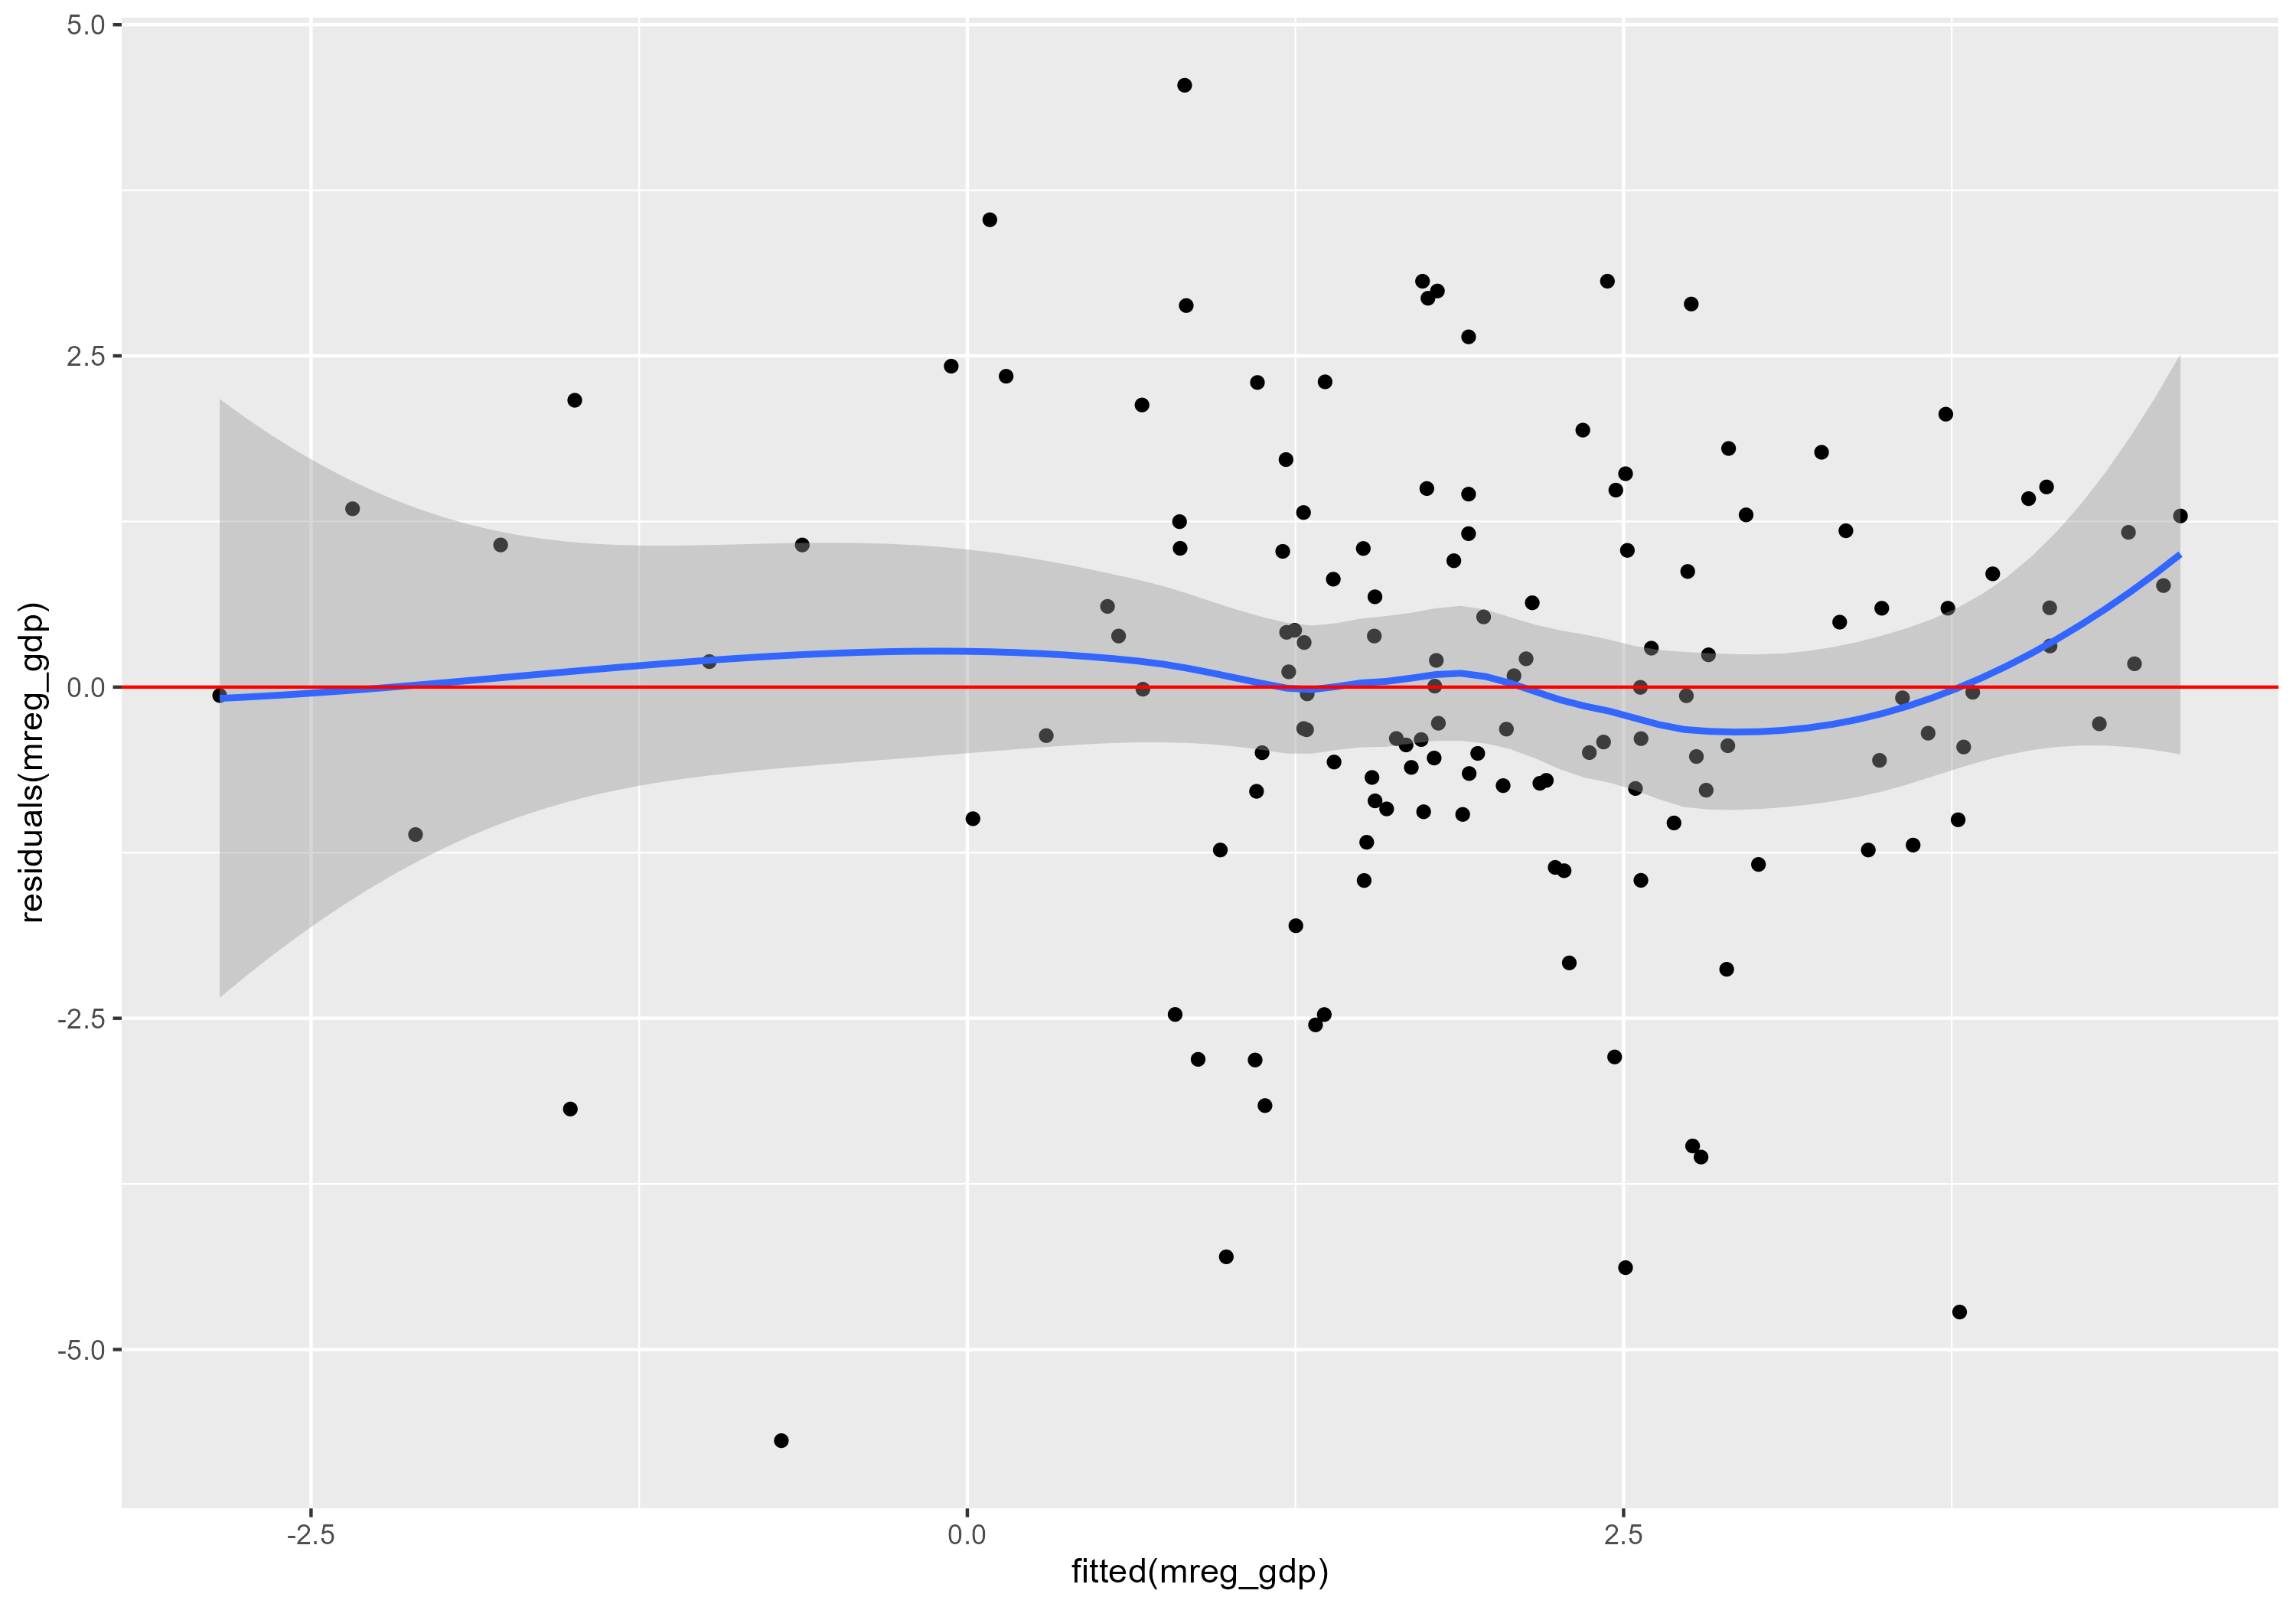
\includegraphics[width=0.5\textwidth]{dokumentobjekter/figurer/linearitet.png}
  \captionof{figure}{Linearitetstest}
  \label{fig:linearitet}
  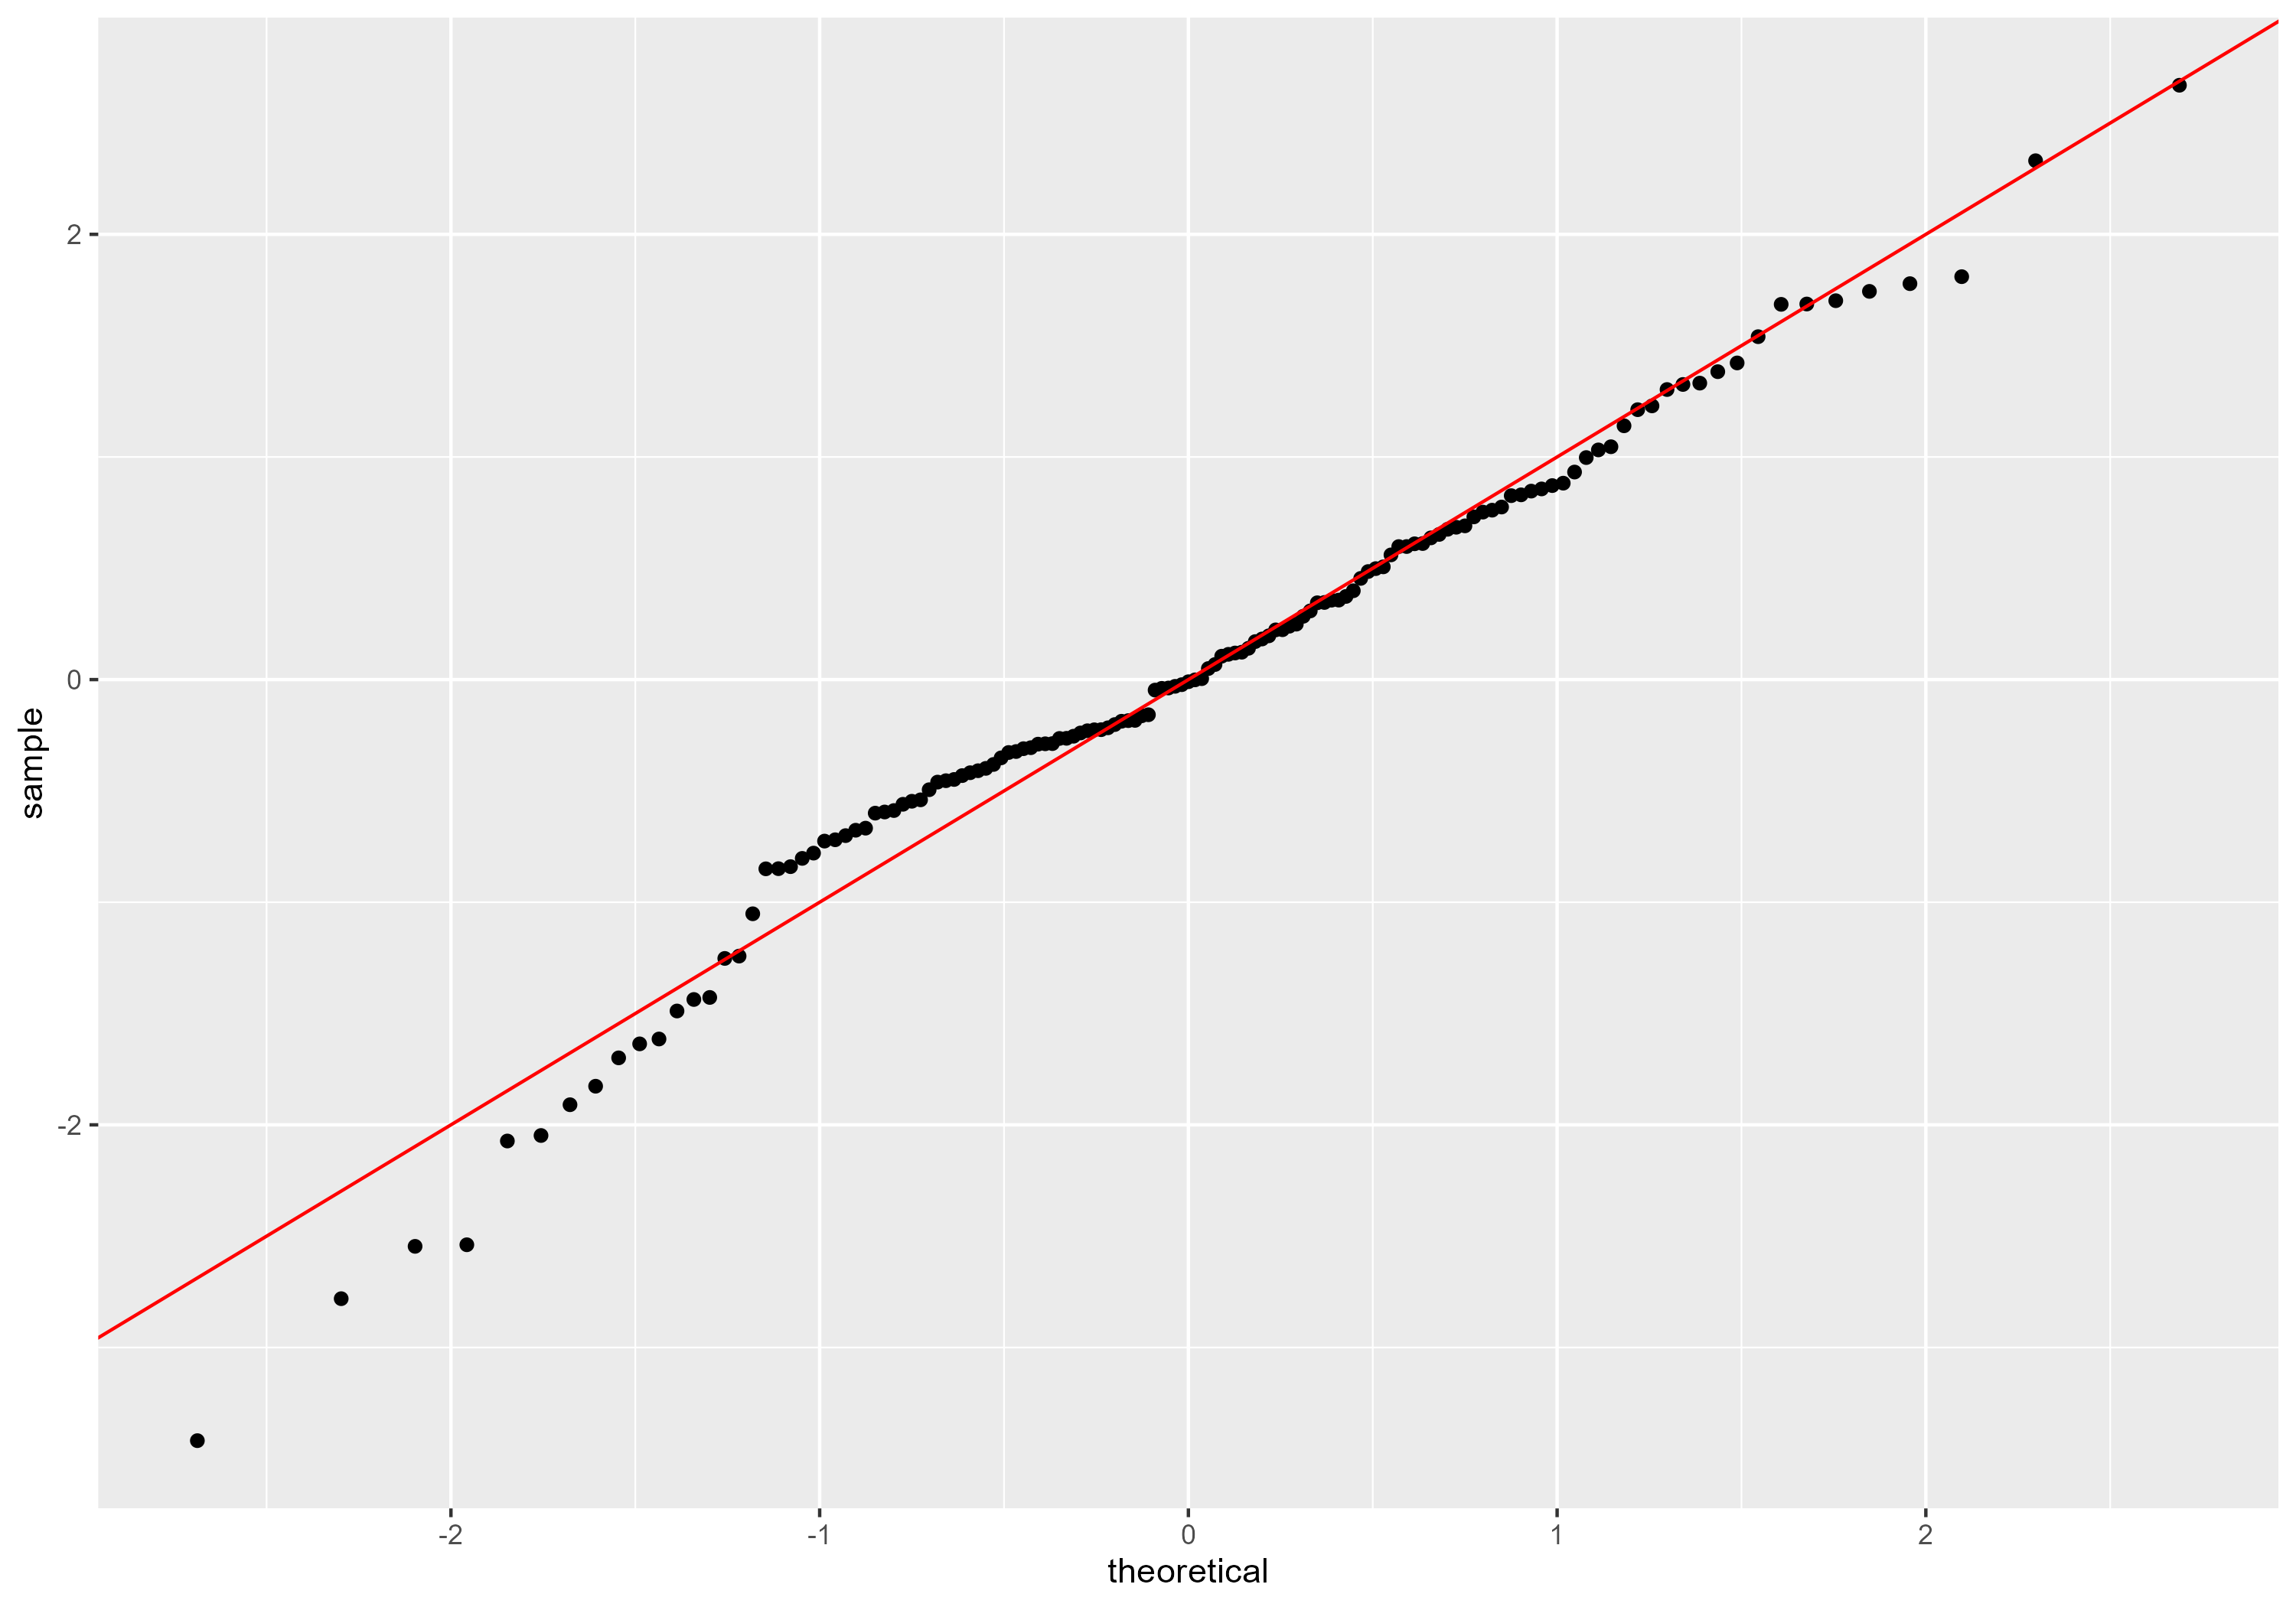
\includegraphics[width=0.5\textwidth]{dokumentobjekter/figurer/normalitet.png}
  \captionof{figure}{Normalitetstest}
  \label{fig:normalitet}
  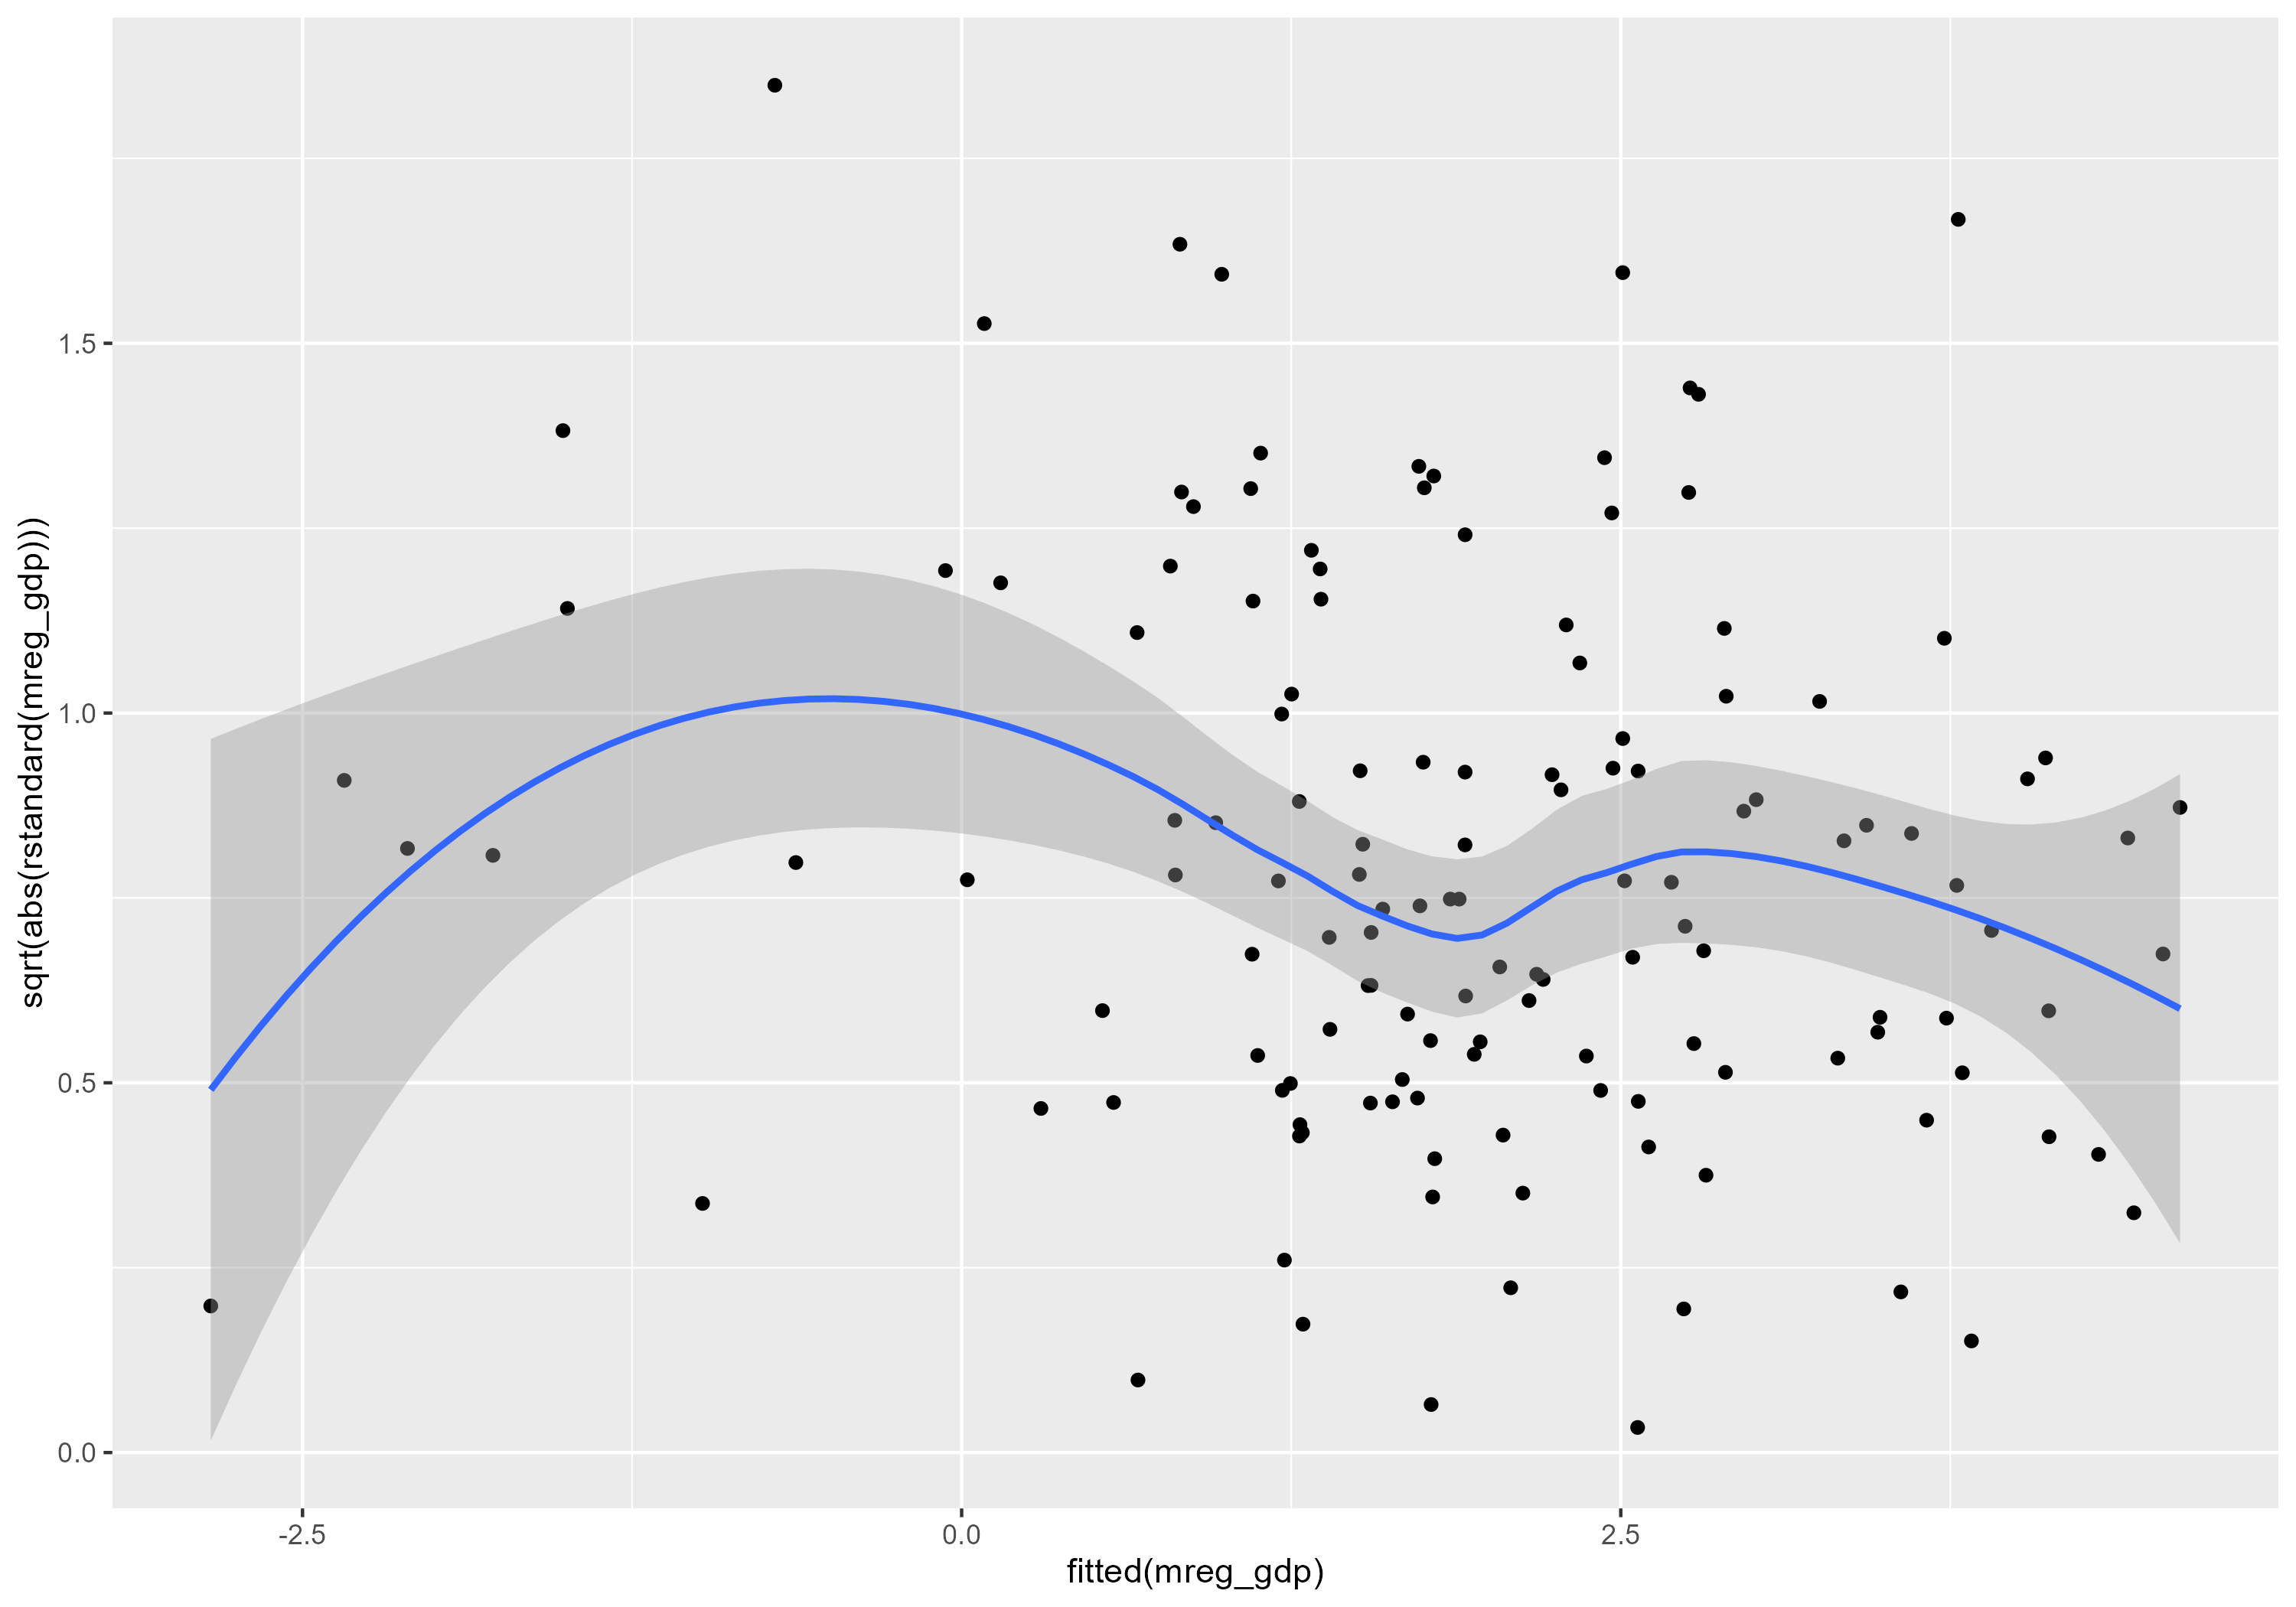
\includegraphics[width=0.5\textwidth]{dokumentobjekter/figurer/homoskedasisitet.png}
  \captionof{figure}{Homoskedasisitetstest}
  \label{fig:homoskedasisitet}
\end{wrapfigure}

Nei å nei. Moderat nesten høy kollinearitet mellom humankapital og
ln\_gdppc0

\paragraph{Linearitet}\label{linearitet}

Vi setter opp en figur med residualene på y aksen og de predikerte
verdiene på x aksen.

Holder seg noe bra men avviker på slutt.

\paragraph{Normalitet}\label{normalitet}

Vi sjekker normaliteten i et kvantil-kvantil plot.

Huff

\paragraph{Homoskedasisitet}\label{homoskedasisitet}

Vi lager en figur der jeg tar kvadratroten av absoluttverdiene til de
standardiserte residualene på y aksen og de predikerte verdiene på x
aksen.

Kan ikke brukes som linjal.

Gjør nå en Non Constant Variance test

\begin{verbatim}
Non-constant Variance Score Test 
Variance formula: ~ fitted.values 
Chisquare = 5.221321, Df = 1, p = 0.022312
\end{verbatim}

Heteroskedastisk?

Modellen har brudd, så dessverre kan vi ikke si at det vi har sett på
har noen statistisk sammenheng.

\clearpage

\section{Referanser}\label{referanser}

\phantomsection\label{refs}
\begin{CSLReferences}{1}{0}
\bibitem[\citeproctext]{ref-worldbank}
\emph{DataBank, the world bank}. (2024).
\url{https://databank.worldbank.org/home.aspx}

\bibitem[\citeproctext]{ref-hess_2016_economic}
Hess, P. N. (2016). \emph{Economic growth and sustainable development}.
Routledge.

\bibitem[\citeproctext]{ref-stargazer}
Hlavac, M. (2022). \emph{Stargazer: Well-formatted regression and
summary statistics tables}. Social Policy Institute.
\url{https://CRAN.R-project.org/package=stargazer}

\bibitem[\citeproctext]{ref-Forelesingsnotat}
Mannberg, A. (2023). \emph{SOK-2011 v2024: Utfodring 2}.
\url{https://uit-sok-2011-v2024.github.io/assets/sok2011_utf2_2024.html}

\end{CSLReferences}

\clearpage

\appendix

\section {Appendix Generell KI bruk}

I løpet av koden så kan det ses mange \# kommentarer der det er skrevet
for eks ``\#fillbetween q1 and q2''. Når vi skriver kode i Visual Studio
Code så finnes det en plugin som heter Github Copilot. Når vi skriver
slike kommentarer så kan den foresøke å fullføre kodelinjene mens vi
skriver de. Noen ganger klarer den det, men andre ikke. Det er vanskelig
å dokumentere hvert bruk der den er brukt siden det ``går veldig fort''
men siden det ikke er fått på plass en slik dokumentasjon så kan all
python kode der det er brukt kommentarer antas som at det er brukt
Github Copilot. Nærmere info om dette KI verktøyet kan ses på
\url{https://github.com/features/copilot}

\href{https://chat.openai.com/share/7251a149-e74a-4599-a550-3f3e95aec068}{Vi
har brukt KI til å skrive sammendrag og kvalitetssikret at det som er
skrevet er korrekt.}

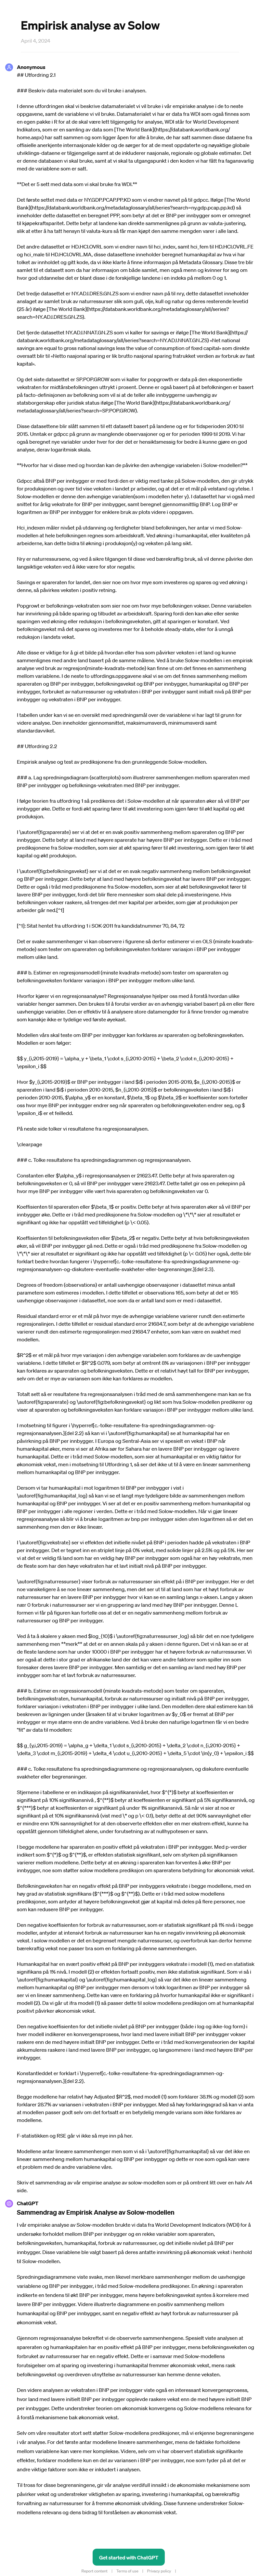
\includegraphics{dokumentobjekter/figurer/chatgpt_sammendrag.png}

\clearpage

\section {Appendix 1.1 KI bruk}

\href{https://chat.openai.com/share/487619f4-de3a-4c08-8932-4317faacd357}{Kandnummer
84 har brukt KI til å få en oversikt på hvordan legge opp skrivingen og
noe struktur}

\includegraphics{dokumentobjekter/figurer/chatgpt_bruk.png}

\section {Appendix Kapittel 1.2 KI bruk}

Ingenting

\label{appendix:appendixkart}

\section {Appendix Kapittel 1.3 KI bruk}

Ingenting



\end{document}
